\documentclass[review]{elsarticle}

\usepackage{lineno,hyperref}
\usepackage{xcolor}
\usepackage{amsmath}
\usepackage{nicefrac}
\usepackage{cleveref}
\usepackage{amssymb}
\usepackage{siunitx}
\usepackage{hyperref}
\usepackage{appendix}
\usepackage{subcaption}
\usepackage{booktabs}
\usepackage{setspace}
%\modulolinenumbers[1]
\journal{International Journal of Hydrogen Energy}
\bibliographystyle{elsarticle-num}
\setlength\parindent{0em}
\usepackage[hang,flushmargin]{footmisc} 






\begin{document}

\begin{frontmatter}

\title{Green hydrogen from hydropower: A non-cooperative open-source modeling approach assessing the profitability gap and future business cases}
\author[1]{Sebastian Zwickl-Bernhard\corref{cor1}}
\ead{zwickl@eeg.tuwien.ac.at}
\author[1]{Hans Auer}
\cortext[cor1]{Corresponding author}
\address[1]{Energy Economics Group (EEG), Technische Universität Wien, Gusshausstrasse 25-29/E370-3, 1040 Wien, Austria}


\begin{abstract}
The core objective of this paper is to investigate a possible future business case for green hydrogen production from hydropower. In particular, the main research question is to find the trade-offs for a run-of-river hydropower plant owner between the currently prevailing business model of wholesale electricity trading and, alternatively, production of green hydrogen. Hence, a bi-level optimization framework (open-source) between a hydropower plant owner (H\textsubscript{2} producer) and a transportation firm (H\textsubscript{2} consumer) is developed. Thereby, the hydropower plant owner acts strategically as the leader in this game and sets the price of green hydrogen. The transportation firm aims for an optimal and cost-minimized coverage of its energy demand and thus chooses between conventional fuels and green hydrogen. The empirical scaling of the numerical example describes Central Western European wholesale electricity market settings. The results indicate that the current market environment and price setup do not allow for profitable green hydrogen production as yet. However, an increasing CO\textsubscript{2} price as the key determining parameter leads to improved competitiveness and expected profitability of the business case studied in this work. In the numerical example examined, a CO\textsubscript{2} price above \SI{245}{EUR \per \tonne} triggers profitability. If decarbonization of the energy systems (in Europe) and the \SI{1.5}{\degreeCelsius} climate targets are taken seriously in policy and decision making, this CO\textsubscript{2} price level can be achieved rather quickly. Future work may address, among others, the following aspects: a more detailed representation of the hydropower plant resource allocation mechanism in the modeling framework, consideration of investment costs of the agents in the objective function, or investigation of the impact on hydrogen production from hydropower in a predominantly renewable energy-based power plant portfolio, and thus regular predatory competition in the (daily) dispatch in periods of favorable renewable resource conditions. 
\end{abstract}


\begin{keyword}
Green hydrogen, Hydropower, Non-cooperative game, Open-Source, Business case, Resource allocation, Opportunity costs
\end{keyword}

\end{frontmatter}

\vspace{0.5cm}
\section{Introduction}
It is indisputable that hydrogen can play a pivotal role in transforming the existing energy systems towards sustainable ones dominated by renewable energy resources \cite{dunn2002hydrogen}. Two reasons are the main drivers for this ambitious perspective. On the one hand, hydrogen offers the opportunity to decarbonize the provision of numerous energy services and sectors \cite{midilli2008hydrogen}. On the other hand, it also adds additional integrated flexibility options, which can be used cross-sectoral and system-overarching \cite{kueppers2021decarbonization}. Implementing flexibility options is particularly inevitable in light of integrating sharply increasing shares of variable renewable energy generation \cite{kroniger2014hydrogen}.\vspace{0.3cm}

Thus, hydrogen deployment is also essential in most of the decarbonization pathways and sustainable economy/society storylines \cite{herbst2021scenario}. Various energy system models already provide comprehensive system analyses, essentially dealing with the required energy technology portfolios and supply options providing future energy demand. The results often include hydrogen as a key technology option to ensure achieving the ambitious climate targets in specific sectors \cite{lux2020supply}. However, one could even go so far as to say that energy system models rely on hydrogen to deliver the various energy services in accordance with the climate targets (e.g., heavy industry \cite{rissman2020technologies} and transport \cite{zhang2016times}).\vspace{0.3cm}

The crucial questions remain: (i) How is hydrogen produced in practice (primary fuels)? (ii) How does the corresponding profitability look like? (iii) And subsequently, how may various business cases succeed, taking into account the individual objectives of the agents involved? The expectation so far mainly is the production of so-called "green" hydrogen\footnote{This work focuses on "green" hydrogen, which is produced by renewable energy resources, notably hydropower, only. Other forms of hydrogen production currently under discussion (e.g., "blue" hydrogen in combination with carbon capture and storage technologies) are not subject of the analysis in this paper.} from renewable energy generation. However, if one examines the available annual full-load hours of the most promising renewable technologies to date such as onshore wind and solar PV, a core handicap becomes visible \cite{ajanovic2018economic}. Both technologies achieve only low annual utilization, and thus, the same applies to on-site infrastructure for hydrogen production \cite{ball2015hydrogen}. The economic viability is getting even worse, if someone argues with renewable energy excess generation only, an argument that has been frequently read these days.\vspace{0.3cm}

Since profitable hydrogen production requires high annual utilization hours, electricity generation technologies scuh as high-efficiency combined cycle gas turbines (CCGTs) and nuclear power plants could be mentioned. However, both technology options cannot meet the criteria to qualify for green hydrogen production. Although the CCGT has already been eliminated as greenhouse gas-emitting technology, nuclear power plants have not. The nuclear industry is in conflict with other policy goals such as sustainable development in general and circular economy/society in particular.\vspace{0.3cm}

To meet the requirements of profitable green hydrogen production, a matching of high annual utilization hours and renewable electricity generation ultimately leaves two technological candidates: offshore wind and hydropower. In particular, in offshore wind technology, high expectations are placed in the future, as it now reaches already up to \SI{5000}{} full-load hours per year (e.g., the floating offshore wind test facility "Hywind Scotland"\footnote{\url{https://www.windtech-international.com/projects-and-contracts/hywind-scotland-reaches-capacity-factor-of-57-1}}). However, (floating) offshore wind, is in a premature stage, but its future seems promising. This leaves the proven hydropower technology to be studied in more detail. In particular, run-of-river hydropower plants deliver throughout the year and are expected to offer themselves as candidates for the new business opportunity of hydrogen production.\vspace{0.3cm}

Thus, the core objective of this paper is to investigate a possible future business case for green hydrogen production from hydropower. In particular, the main research question is to find the trade-offs for a run-of-river hydropower plant owner between trading of electricity (e.g., forward/future electricity contracts or at the day-ahead spot market) and, alternatively, production of green hydrogen. The optimal exploitation and allocation of hydropower resources plays a key role in the analysis. Equally important is the impact of different $CO_2$ prices on the profitabilty of electricity trading and green hydrogen production.\vspace{0.3cm} 

The method applied to answer the research question is the development of a non-cooperative optimization model. Thereby, the bi-level optimization framework is implemented with a single leader ($H_2$ producer) and follower ($H_2$ consumer). Both agents are profit oriented. Thus, their objectives are maximizing revenues and minimizing total costs, respectively. The non-cooperative game-theoretical approach ensures transferability of the results in reality and applicability to real-world use cases.\vspace{0.3cm} 

The case study analyzed is a non-cooperative game between a run-of-river hydropower plant owner and a company in the freight transport business. The first one serves as the leader in this game and acts as the price setter for green hydrogen. The latter one is the follower and aims for an optimal and cost-minimized coverage of its energy demand (e.g., for fueling its vehicle fleet). Thereby, the transportation firm decides among conventional fossil fuels or hydrogen. Simultaneously, the leader has complete information and anticipates the green hydrogen price and the resource allocation to maximize its revenues.\vspace{0.3cm} 

The paper is organized as follows. Section \ref{stateoftheart} summarizes the current state-of-the-art in literature and outlines the present study's own contribution beyond the state-of-the-art. Section \ref{methodology} presents the methodology and the developed mathematical framework, followed by the detailed numerical example description in Section \ref{numerical}. Section \ref{results} presents the results of this work, including sensitivity analyses of key determining parameters. Section \ref{conclusion} discusses the results, concludes the work, and outlines possible future research.

\section{State-of-the-art and progress beyond}\label{stateoftheart}
The following state-of-the-art overview summarizes key findings in literature in the context of this work's scope. Hence, this section is split into three main parts. Section \ref{state1} elaborates generally on the importance of hydrogen in a sustainable energy system. Closely related to this are the areas of application. On this basis, Section \ref{state2} addresses the different energy resources and technology options for producing hydrogen. Here, the central focus is put on the expected profitability and economic viability. Finally, Section \ref{state3} covers the different methodological approaches to energy system modeling and distinguishes between system analysis and agent-based modeling. In particular, the latter addresses cooperative and non-cooperative games of the agents involved in decision making. 

\subsection{The role of hydrogen in sustainable energy systems}\label{state1}
Many studies have elaborated on the role and importance of hydrogen in energy systems \cite{midilli2005hydrogen}. In particular, recent studies address the opportunities of hydrogen in a sustainable energy supply \cite{moller2017hydrogen}. Hopeful signs, however, are by no means a new phenomenon but have been observed already for some decades \cite{dunn2002hydrogen}. The reason for this is that hydrogen is a technology already well-understood \cite{momirlan2002current}. However, hydrogen has not yet fulfilled its expectations, and its role remains ambiguous. On the one hand, it is a viable alternative to other energy carriers \cite{johnston2005hydrogen} (e.g., conventional fuels); on the other hand, it is a technology that has barely penetrated the market so far. In addition, the hydrogen technology is still associated with uncertainties in the acceptance \cite{da2017hydrogen}, not least because a limited efficiency of hydrogen production has been achieved so far only \cite{page2009system}. Notwithstanding this, the future potential of hydrogen has to be balanced against possible benefits and system improving effects \cite{mcpherson2018role}, such as overcoming the fossil fuel dependencies and thus accelerating the decarbonization of the energy systems \cite{lux2020supply} as well as ultimately striving for the achievements of the climate targets \cite{chapman2020societal}.\vspace{0.3cm}

In literature, high potentials for substitution of conventional fuels by hydrogen are identified in many sectors \cite{burandt2019decarbonizing} and energy services \cite{mouli2021mapping}. Exemplarily, feasible real-life applications in the transportation sector are presented in \cite{zhang2016times}, whereas \cite{auer2020development} focuses on the freight transport sector in particular. In addition, there are considerable potentials in the heavy industries (e.g., process heat) becoming increasingly important. The work in \cite{rissman2020technologies} concludes that hydrogen deployment must be considered mandatory in the heavy industry in order to meet the long-term goals of a net-zero emission economy. 


\subsection{Sources for hydrogen production in a historical context}\label{state2}
There are a number of different possibilities for the production of hydrogen. This Section \ref{state2} primarily discusses the energy resources for hydrogen production in a historical context. Others such as the methods or technical aspects of the hydrogen production process are not covered in what follows. In this respect, reference is made to specific scientific literature (see exemplarily in \cite{dincer2015review}).\vspace{0.3cm}

At the outset, there was the common perception to produce hydrogen from fossil fuels. The work in \cite{steinberg1989modern} and \cite{kathe2016hydrogen} clearly shows that gas, oil, and coal offer the possibility for a profitable hydrogen production. However, it should be explicitly noted, that even at that time, when fossil fuel-based technologies were designated as prospective, scientific studies already claimed for a $CO_2$ emission-free hydrogen production \cite{muradov1993produce}. This has also prompted the nuclear industry to promote the benefits of its technology for emission-free and economic viable hydrogen production on a large-scale. A number of publications over the last decades point to this fact. Yalcin \cite{yalcin1989review} published a fundamental review of nuclear hydrogen production already in the late 1980s. Kruger \cite{kruger2009nuclear} and Yildiz et al. \cite{yildiz2006efficiency} emphasized the role of nuclear power as an appropiate and highly efficient technology for hydrogen production. Notwotny et al. \cite{nowotny2016towards} focus in their work on nuclear-based hydrogen toward sustainable energy provision. And recently, the authors in \cite{karaca2020life} conducted a life cycle assessment comparison of nuclear-based hydrogen production options.\vspace{0.3cm}

Today's perspective of hydrogen market integration not only requires emission-free production but is also intended to replace the gas-emitting technologies in the energy system at the same time. Then only global fossil fuel consumption \cite{midilli2008hydrogen} and hence global $CO_2$ emissions can be reduced efficiently and effectively. Although nuclear power plants could produce emission-free hydrogen, there has always been both the latent nuclear accident risk and the unresolved question of the final disposal of radioactive waste. These concerns do not match with the emerging ambitions to establish a recycling economy and general sustainable development goals in society \cite{sdg2018sustainable}. Against this background, hydrogen production from renewable resources seems to be more promising.\vspace{0.3cm} 

In the light of sustainable energy system transformation, mainly (onshore) wind and solar PV have been analyzed so far as technology options for hydrogen production \cite{nematollahi2019techno}, basically because hydrogen as an energy storage technology offers flexibility options to its variable/fluctuating electricity generation \cite{mcpherson2018role}. In case of wind power generation, forecasting errors can be compensated \cite{kroniger2014hydrogen}, and/or the curtailment of excess electricity generation from wind \cite{mcdonagh2020hydrogen} and solar PV \cite{wu2020investment} can be prevented \cite{mcdonagh2019electrofuels}. The scientific contributions also consider hydrogen flexibility options in local energy systems, such as microgrids \cite{li2021multiple, bornapour2017optimal, li2017sizing}. However, from an economic perspective, hydrogen production from onshore wind and solar PV has structural limitations regardless of the aggregation level in the energy system. The main problem relates to the resource-dependent low annual utilization hours \cite{moraes2018comparison, ajanovic2018economic}. This dilemma is expected to be overcome in the future with offshore wind \cite{leahy2020development, mcdonagh2020hydrogen}, notably the promising floating offshore wind technology. As already mentioned in the introduction of this work, first test site parameters of the floating offshore wind technology justify confidence for the future.\vspace{0.3cm}

Eventually, along with the elaboration on the advantages and limitations of renewable energy-based hydrogen production in scientific literature in the past comes renewable technology options being subjected to further investigations. However, most of them have the character of niche applications and not yet considered suitable for large-scale supply \cite{glenk2019economics}. Exemplarily, the work in \cite{cao2020biorenewable} presents a comprehensive review and future prospects on hydrogen production through biomass gasification. This is in line also with the results in \cite{kelly2007potential}. Nevertheless, biomass as a renewable energy source hardly will lead to a competitive large-scale green hydrogen production in the future.\vspace{0.3cm}

Last but not least, hydropower technology remains. Not only is it a well-established and understood renewable technology, but it also has none of the disadvantages and/or limitations mentioned so far in the context of hydrogen production. Therefore, hydropower-based hydrogen production is a serious option that should be given more attention. The reason for little attention so far has been that the direct feeding of hydropower generation into the electricity grid and the exclusive use for electricity-specific energy services of customers are the most profitable business cases for all agents involved in the energy supply chain. This, however, could change in the future during massive excess electricity generation solely from renewable technologies (e.g., hydropower, wind, and solar PV), where a certain degree of predatory competition cannot be ruled out in periods of favorable resource availability. Moreover, an expected increasing future $CO_2$ price also justifies thinking beyond the traditional business models of hydropower producers. In this context, scarce scientific literature has so far investigated how flexible hydrogen production can also improve the optimal operation of hydropower plants \cite{lu2015optimal} and enhances the value of hydropower in superior networks as well as congested transmission grids \cite{bodal2020value}. However, the focus in this work is not on technical or energy system-related benefits associated with hydrogen production but on its profitability from hydropower resources. For a techno-economic assessment of hydrogen production from hydropower, refer to \cite{olateju2016techno}. By studying the rare literature so far and anticipating future developments governing decarbonization of energy systems, one may conclude that hydropower is the most promising renewable energy technology option for green hydrogen production. Nonetheless, there is a lack of scientific contributions that address in detail possible future business cases, the existing profitability gap, and the corresponding trade-offs of hydropower-based green hydrogen production.

\subsection{Modeling approaches and allocation of limited/distributed resources}\label{state3}
Most of the already acknowledged scientific studies above analyze hydrogen production and deployment from a system analysis or energy planning perspective emphasizing mainly techno-economic aspects. Furthermore, the recent work in \cite{qolipour2017techno} provides another comprehensive techno-economic feasibility study of hydrogen. At the same time, and as indicated above, the energy resources for the hydrogen production are again mainly onshore wind and solar PV (also in \cite{wu2020cooperative}). In addition, some works also elaborate on the large-scale potentials of hydrogen (e.g., in a low-carbon European energy system using cost optimization in \cite{blanco2018potential}). Besides, the energy system analysis in \cite{lund2009energy} emphasizes the role of hydrogen in a \SI{100}{\%} renewable energy system country study.\vspace{0.3cm}

However, there can be situations where reasons for agent-based strategic behavior necessitate game-theoretical analysis approaches \cite{wei2017stackelberg}. Specifically, in the context of revenue and profit maximization of existing business models, such as those for hydropower plant operators, this strategic consideration is necessary and appropriate \cite{fleten2007stochastic}. In the context of game theory modeling from an overall perspective, the reader is referred to the fundamental work in \cite{gintis2000game}.\vspace{0.3cm}

In general, strategic behavior of agents in the energy system can be observed at various scales. The work in \cite{girones2015strategic} provides a modeling framework to aid decision making on large-scale energy systems. On the basis of high spatial granularity, the work in \cite{khojasteh2020robust} investigates hydrogen-based operation strategies for a microgrid. Game theoretical analysis of an agent's behavior on a local or neighborhood level is addressed in \cite{jing2018multi} and \cite{fleischhacker2018sharing}. In this context, the authors in \cite{fernandez2018game} conducted a game-theoretic analysis of optimal demand-side energy management on the neighborhood level incorporating high shares of renewable resources. The work in \cite{jing2018multi} presents game-theory inspired local energy resource allocation constraints taking into account multi-objective optimization for an urban neighborhood. Recently, Luo et al. \cite{luo2020energy} published a three-level Stackelberg game approach investigating optimal energy scheduling. All these references cited above do not claim for completeness of scientific studies dealing with game-theoretical approaches in energy system modeling. Instead, selected studies are mentioned to indicate the relevance of game-theoretical approach analysis in the context of this work's focus. It has to be pointed out, however, that there is a lack of scientific studies dealing with hydrogen production from renewable energy resources off the surplus production argument in general and from hydropower resources in particular.

\subsection{Progress beyond state of the art}
The progress beyond the state of the art and thus novelty of this work contribute at least in the following dimensions:

\begin{itemize}
	\item This work conducts a thorough analysis of hydropower-based green hydrogen production. In this context, the focus is directed on possible self-sustaining business models of green hydrogen production for run-of-river hydropower plant owners, who so far predominantly have been focusing purely on the production of electricity, feeding electricity into the grid, and selling electricity in the electricity market. Thus, possible green hydrogen business cases are revealed in this work, going beyond the myth of green hydrogen production based on renewable energy surplus generation from (onshore) wind and solar PV, which still face the inherent problem of low achievable annual capacity factors. 
	
	\item The modeling framework (open-source) determines the optimal resource allocation of a hydropower plant owner between electricity trading on the wholesale markets (day-ahead spot market and forward/futures market) and green hydrogen production. Thereby, the framework setup consists of two profit-maximizing agents, taking into account a bilateral non-cooperative game between a hydropower plant owner (leader, or the $H_2$ producer) and a transportation firm (follower, or the $H_2$ consumer). In particular, the key parameters determining the strategic behavior of the agents are the generation shadow price, opportunity costs, and the $CO_2$ price.  
	
	\item On the basis of the results developed in this work, a temporal frame of profitable green hydrogen production from hydropower is provided by examining the implications of different $CO_2$ prices on the optimal resource allocation. The calculated $CO2$ prices of this work are matched with determined $CO2$ prices in different European energy system scenario studies (taking into account the decarbonization needs for complying to the ambitious \SI{1.5}{\degreeCelsius} climate targets) and thus enable a temporal framing of the expected profitability of hydropower-based green hydrogen production in the upcoming decades. 
\end{itemize}
\newpage
\section{Methodology}\label{methodology}
This section explains the methodology applied in this work. Since the lower level's ($H_2$ consumer) mathematical framework is embedded in that of the upper level ($H_2$ producer), Section \ref{sec:lower} describes the follower's (non-linear) optimization problem first. This includes the Karush-Kuhn-Tucker (KKT) conditions and its strong duality formulation. Section \ref{sec:leader} presents the leader's mathematical framework. Finally, Section \ref{sec:bi_level} concludes with the description of the full bi-level optimization problem.

\subsection{Follower's mathematical framework}\label{sec:lower}

\paragraph{Objective function} The follower aims to minimize total costs to cover its demand. Therefore, the objective function can be written as follows: 

\begin{align}\label{objective}
\underset{\b{$x$}}{\mathrm{min~}}  \sum_{t} q_{t}^{con} \cdot p_{t}^{con} + q_{t}^{H_2} \cdot p_{t}^{H_2} +  q_{t}^{CO_2} \cdot p_{t}^{CO_2}
\end{align}

where $ q_{t}^{con}$ is quantity and  $ p_{t}^{con}$ the price of conventional fuels at time step t. Accordingly, $q_{t}^{H_2}$ and $p_{t}^{H_2}$ are for hydrogen and $q_{t}^{CO_2}$ and $p_{t}^{CO_2}$ are for CO\textsubscript{2} emissions. In addition, $\b{$x$}$ contains the decision variables of the follower and can be represented as a vector. 

\paragraph{Decision variables} To enhance readability, the decision variables are summarized in the decision variable vector  $\b{$x$}$. This can be written as follows:

\begin{align}
\b{$x$}=[q_{t}^{con},q_{t}^{H_2},q_{t}^{CO_2}]
\end{align}

\paragraph{Parameters} Analogous to the decision variable vector, all parameters are combined into the parameter vector $\b{$d$}$ as follows:

\begin{align}
\b{$d$}=[p_{t}^{con},p_{t}^{H_2},p_{t}^{CO_2}, \alpha^{con}, \beta^{con}, q_{t}^{load}]
\end{align}

where $\alpha^{con}$ is the emission factor, $\beta^{con}$ the energy density factor of conventional fuels and $q_{t}^{load}$ the quantity of demand at time step $t$.

\paragraph{Constraints} Equation (\ref{equ_follower_load}) describes the load satisfaction constraint at all time steps $t$. Note that $\lambda_{t}^{load}$ is the dual variable. $\beta^{con}$ ensures unit comparability for conventional fuels and hydrogen.

\begin{align}\label{equ_follower_load}
q_{t}^{load} - \beta^{con} \cdot q_{t}^{con} - q_{t}^{H_2} = 0 \quad :\lambda_{t}^{load} \quad (\forall t)
\end{align}

Equation (\ref{equ_follower_emissions}) equals the quantity of CO\textsubscript{2} greenhouse gas emissions at each time step $t$ (due to $q_{t}^{con}$). Again $\lambda_{t}^{CO_2}$ is the dual variable of Equation \labelcref{equ_follower_emissions}.

\begin{align}\label{equ_follower_emissions}
q_{t}^{CO_2} - \alpha^{con} \cdot q_{t}^{con} = 0 \quad :\lambda_{t}^{CO_2} \quad (\forall t)
\end{align}

In addition, Equation (\ref{equ_follower_nonnegative}) ensures non-negativity of the decision variables and introduces the corresponding dual variables $\mu_t^{con}$, $\mu_t^{H_2}$, and $\mu_t^{CO_2}$.

\begin{align}\label{equ_follower_nonnegative}
\begin{aligned}
q_{t}^{con} \geq 0 & \quad:\mu_t^{con} & \quad(\forall t)\\
q_{t}^{H_2} \geq 0 & \quad:\mu_t^{H_2} & \quad(\forall t)\\
q_{t}^{CO_2} \geq 0 & \quad:\mu_t^{CO_2} & \quad(\forall t)
\end{aligned}
\end{align}

\subsubsection{Karush-Kuhn-Tucker conditions}
% notwendige und hinreichende Bedingungen für KKT conditions
The well-known KKT conditions are used to transform the follower's optimization framework as linear constraints into the leader's optimization framework. Therefore, the Lagrangian function is formulated as follows:

\begin{align}
\begin{split}
\mathcal{L}(\b{$x$}, \b{$\lambda$}, \b{$\mu$}) &=\sum_{t} q_{t}^{con} \cdot p_{t}^{con} + q_{t}^{H_2} \cdot p_{t}^{H_2} + q_{t}^{CO_2} \cdot p_{t}^{CO_2}\label{equ_follower_Lagrangian}\\
& \quad + \lambda_{t}^{load} \cdot (q_{t}^{load} - \beta^{con} \cdot q_{t}^{con} - q_{t}^{H_2})\\
& \quad + \lambda_{t}^{CO_2} \cdot (q_{t}^{CO_2} - \alpha^{con}\cdot q_{t}^{con})\\
& \quad + \mu_t^{con} \cdot (-q_{t}^{con}) + \mu_t^{H_2} \cdot (-q_{t}^{H_2}) + \mu_t^{CO_2} \cdot (-q_{t}^{CO_2})
\end{split}
\end{align}
where $\b{$\lambda$}$ contain the equality dual variables in Equation \labelcref{equ_follower_load} and \labelcref{equ_follower_emissions} and $\b{$\mu$}$ the inequality dual variables in Equation \labelcref{equ_follower_nonnegative}. Note that $\b{$\lambda$}$ is $\in$ $\mathbb{R}$. Derived from the Lagrangian function in the prior equation, the KKT conditions can be written as follows:
\begin{align}\label{h1}
\frac{\partial \mathcal{L}}{\partial q_{t}^{con}} = p_{t}^{con} - \beta^{con} \cdot \lambda_t^{load} - \alpha^{con}\cdot \lambda_{t}^{CO_2}-\mu_t^{con} = 0 \quad (\forall t)
\end{align}
\begin{align}\label{h2}
\frac{\partial \mathcal{L}}{\partial q_{t}^{H_2}} = p_{t}^{H_2} - \lambda_t^{load} -\mu_t^{H_2} = 0 \quad (\forall t)
\end{align}
\begin{align}\label{h3}
\frac{\partial \mathcal{L}}{\partial q_{t}^{CO_2}} = p_{t}^{CO_2} + \lambda_t^{CO_2} -\mu_t^{CO_2} = 0 \quad (\forall t)
\end{align}
\begin{align}
0 \leq \mu_t^{con} \bot -q_{t}^{con} \leq 0 \quad (\forall t) \label{CC1}\\
0 \leq \mu_t^{H_2} \bot -q_{t}^{H_2} \leq 0 \quad (\forall t) \label{CC2}\\
0 \leq \mu_t^{CO_2} \bot -q_{t}^{CO_2} \leq 0 \quad (\forall t) \label{CC3}
\end{align}
The complementarity conditions in Equations \labelcref{CC1,CC2,CC3} are linearized using the well-known linear expressions (see in \cite{ruiz2009pool}) as follows:
\begin{align}\label{cc}
\begin{aligned}
0 \leq \mu_{t}^{con} \leq M^{con} \cdot u_{t}^{con} \quad (\forall t)\\
0 \leq q_{t}^{con} \leq M^{con} \cdot (1-u_{t}^{con}) \quad (\forall t)\\
0 \leq \mu_{t}^{H_2} \leq M^{H_2} \cdot u_{t}^{H_2}\quad (\forall t)\\
0 \leq q_{t}^{H_2} \leq M^{H_2} \cdot (1-u_{t}^{H_2})\quad (\forall t)\\
0 \leq \mu_{t}^{CO_2} \leq M^{CO_2} \cdot u_{t}^{CO_2}\quad (\forall t)\\
0 \leq q_{t}^{CO_2} \leq M^{CO_2} \cdot (1-u_{t}^{CO_2})\quad (\forall t)
\end{aligned}
\end{align}

where $u_{t}^{con}$, $u_{t}^{H_2}$, and $u_{t}^{CO_2}$ are binary decision variables. They are summarized in the following section by the binary decision variable vector $\b{u}$.

\subsubsection{Strong duality}
The Lagrangian function and strong duality are used to linearize non-linear terms in the bi-level optimization problem (for more details, see Section \ref{sec:leader}). Therefore, the dual objective function of the follower's optimization problem can be written as follows:

\begin{align}\label{duality}
	\underset{\b{$\lambda$}, \b{$\mu$}}{\mathrm{max~}} [\underset{\b{$x$}}{\mathrm{min~}} \mathcal{L}(\b{$x$}, \b{$\lambda$}, \b{$\mu$})] =\underset{\b{$\lambda$}, \b{$\mu$}}{\mathrm{max~}} \left(- \sum_{t} \lambda_{t}^{load}\cdot q_{t}^{load}\right)
\end{align}

Note that in the optimal solution, equality applies between Equations \labelcref{duality} and \labelcref{objective}.

\subsection{Leader's mathematical framework}\label{sec:leader}
The leader aims to maximize total revenues. Therefore, the objective function can be written as follows: 

\begin{align}
\underset{\bar{y}}{\mathrm{max~}} = \sum_{t} q_{t}^{spot}\cdot p_{t}^{spot}+q_{t}^{future}\cdot p_{t}^{future}+q_{t}^{H_2}\cdot p_{t}^{H_2}
\end{align}

where $q_{t}^{spot}$ is the quantity of electricity sold at the day-ahead spot market, $p_{t}^{spot}$ the day-ahead spot market price, $q_{t}^{future}$ the quantity of the future electricity contract, and $p_{t}^{future}$ the future electricity contract price at time step $t$.

\paragraph{Decision variable vector} The decision variable vector $\bar{y}$ of the leader can be written as follows:

\begin{align}
\bar{y}=[q_{t}^{spot},q_{t}^{future},q_{t}^{Curtail}, p_{t}^{H_2}]
\end{align}

where $q_{t}^{Curtail}$ is the quantity of curtailment at time step $t$.

\paragraph{Parameters}
The leader's parameter vector $\bar{d}$ can be written as follows:
\begin{align}
\bar{d}=[p_{t}^{spot},p_{t}^{future},q_{t}^{gen}, \tilde{q}_{t}^{base}, \eta^{H_2}]
\end{align}

where $q_{t}^{gen}$ contains the electricity generation at time step $t$ and $\tilde{q}_{t}^{base}$ the constant electricity generation band that can be utilized either as a future electricity contract or for the hydrogen production. $\eta^{H_2}$ is the efficiency of the hydrogen production. 

\paragraph{Constraints} Equality \labelcref{L1} equals electricity generation and used quantities for each time step $t$. Equations \labelcref{L3}-\labelcref{L7} ensure a constant future electricity contract and hydrogen production at each time step $t$. In addition, Equation \labelcref{L7} ensures that only the available constant band of electricity generation can be used for the future electricity contract and hydrogen production at each time step $t$. Equation \labelcref{L8} is the non-negative inequality constraint of the leader's decision variables for each time step $t$.

\begin{align}\label{L1}
	q_{t}^{spot} + q_{t}^{curtail} + q_{t}^{future} + \nicefrac{q_{t}^{H_2}}/{\eta^{H_2}} - q_{t}^{gen} = 0 \quad (\forall t)
\end{align}

\begin{align}\label{L3}
\begin{aligned}
q_{t}^{future} - q_{t-1}^{future} = 0 \quad (\forall t \backslash \{t_0\})\\
q_{t}^{future} - q_{t_{end}}^{future} = 0 \quad (\forall t \in \{t_0\})
\end{aligned}
\end{align}

\begin{align}\label{L5}
\begin{aligned}
q_{t}^{H_2} - q_{t-1}^{H_2} = 0 \quad (\forall t \backslash \{t_0\})\\
q_{t}^{H_2} - q_{t_{end}}^{H_2} = 0 \quad (\forall t \in \{t_0\})
\end{aligned}
\end{align}

\begin{align}\label{L7}
\nicefrac{q_{t}^{H_2}}{\eta^{H_2}} + q_{t}^{future} - \tilde{q}^{base} = 0 \quad (\forall t)
\end{align}

\begin{align}\label{L8}
\begin{aligned}
q_{t}^{spot} \geq 0 \quad (\forall t)\\
q_{t}^{future} \geq 0 \quad (\forall t)\\
q_{t}^{curtail} \geq 0 \quad (\forall t)\\
p_{t}^{H_2} \geq 0 \quad (\forall t)
\end{aligned}
\end{align}

\subsection{Bi-level optimization problem}\label{sec:bi_level}
Using the mathematical formulation introduced above, the KKT conditions, and strong duality, the bi-level optimization problem can be written as follows:

\begin{align}\label{bi_1}
\begin{split}
\underset{\bar{y}, \b{x}, \b{$\lambda$}, \b{$\mu$}}{\mathrm{max~}}&\sum_{t} q_{t}^{spot}\cdot p_{t}^{spot}+q_{t}^{future}\cdot p_{t}^{future}\\
& - \lambda_{t}^{load} \cdot q_{t}^{load} + q_{t}^{con}\cdot p_{t}^{con}+q_{t}^{CO_2}\cdot p_{t}^{CO_2}\\
\end{split}
\end{align}

\begin{align}\label{bi_2}
\begin{aligned}
\mathrm{s.t.~} \labelcref{L1}-\labelcref{L8}\\
\labelcref{h1}-\labelcref{h3}\\ 
\labelcref{cc}
\end{aligned}
\end{align}

Owing to some of the KKT conditions and the strong duality formulation, this model is a mixed-integer linear program. Thus, it can be efficiently solved with usual methods (see also Section \ref{numerical}).

\section{Numerical example}\label{numerical}
To illustrate a potential application of the proposed bi-level optimization framework, a bilateral game between a run-of-river hydropower plant owner (leader) and a freight transportation firm (follower) in Austria is applied. Austria has a long tradition and history of hydropower production, which is expressed in Austria's potentially ambitious perspectives of green hydrogen production. Note that owing to the generic model formulation, different hydrogen consumers can be considered. The framework is also transferable to other sectors or regions and explicitly includes the heavy industry and other large consumers worldwide. 

\paragraph{Empirical settings} The day-ahead spot market prices are included as $p_{t}^{spot}$ for two illustrative consecutive days of May $29$ and 30, 2020 \cite{EEG} (original data inputs from  EPEX Spot\footnote{EPEX spot is the Central Western European wholesale electricity market place.}). The electricity generation profile of the run-of-river hydropower plant is taken from \cite{EEG}. The (base) future electricity contract price is \SI{45}{EUR \per MWh} \cite{EEG} (original data inputs from EEX\footnote{EEX is the Austrian wholesale electricity market place, strongly linked to the EPEX price indices.}). The conventional fossil fuel price is \SI{0.112}{EUR\per MWh} \cite{EEG} (original inputs from \textit{Global Petrol Prices}\footnote{\url{https://www.globalpetrolprices.com/}}). As an example, diesel serves as conventional reference fossil fuel in this work. The CO\textsubscript{2} price is \SI{38}{EUR\per t} \cite{EEG} (original inputs from \textit{Ember}\footnote{\url{https://ember-climate.org/data/}}) and the emission factor $\alpha^{con}$ is \SI{0.27}{\tonne \per MWh} \cite{EEG}. These settings are illustrated in Figure \ref{fig:prices}. The load quantity is \SI{10}{MWh} for each time step $t$. Thus, the transportation firm's demand is equal to a \SI{96~000}{km} drive per day. For further empirical details, please see \ref{app:a}.

\begin{figure}[h]
	\centering
	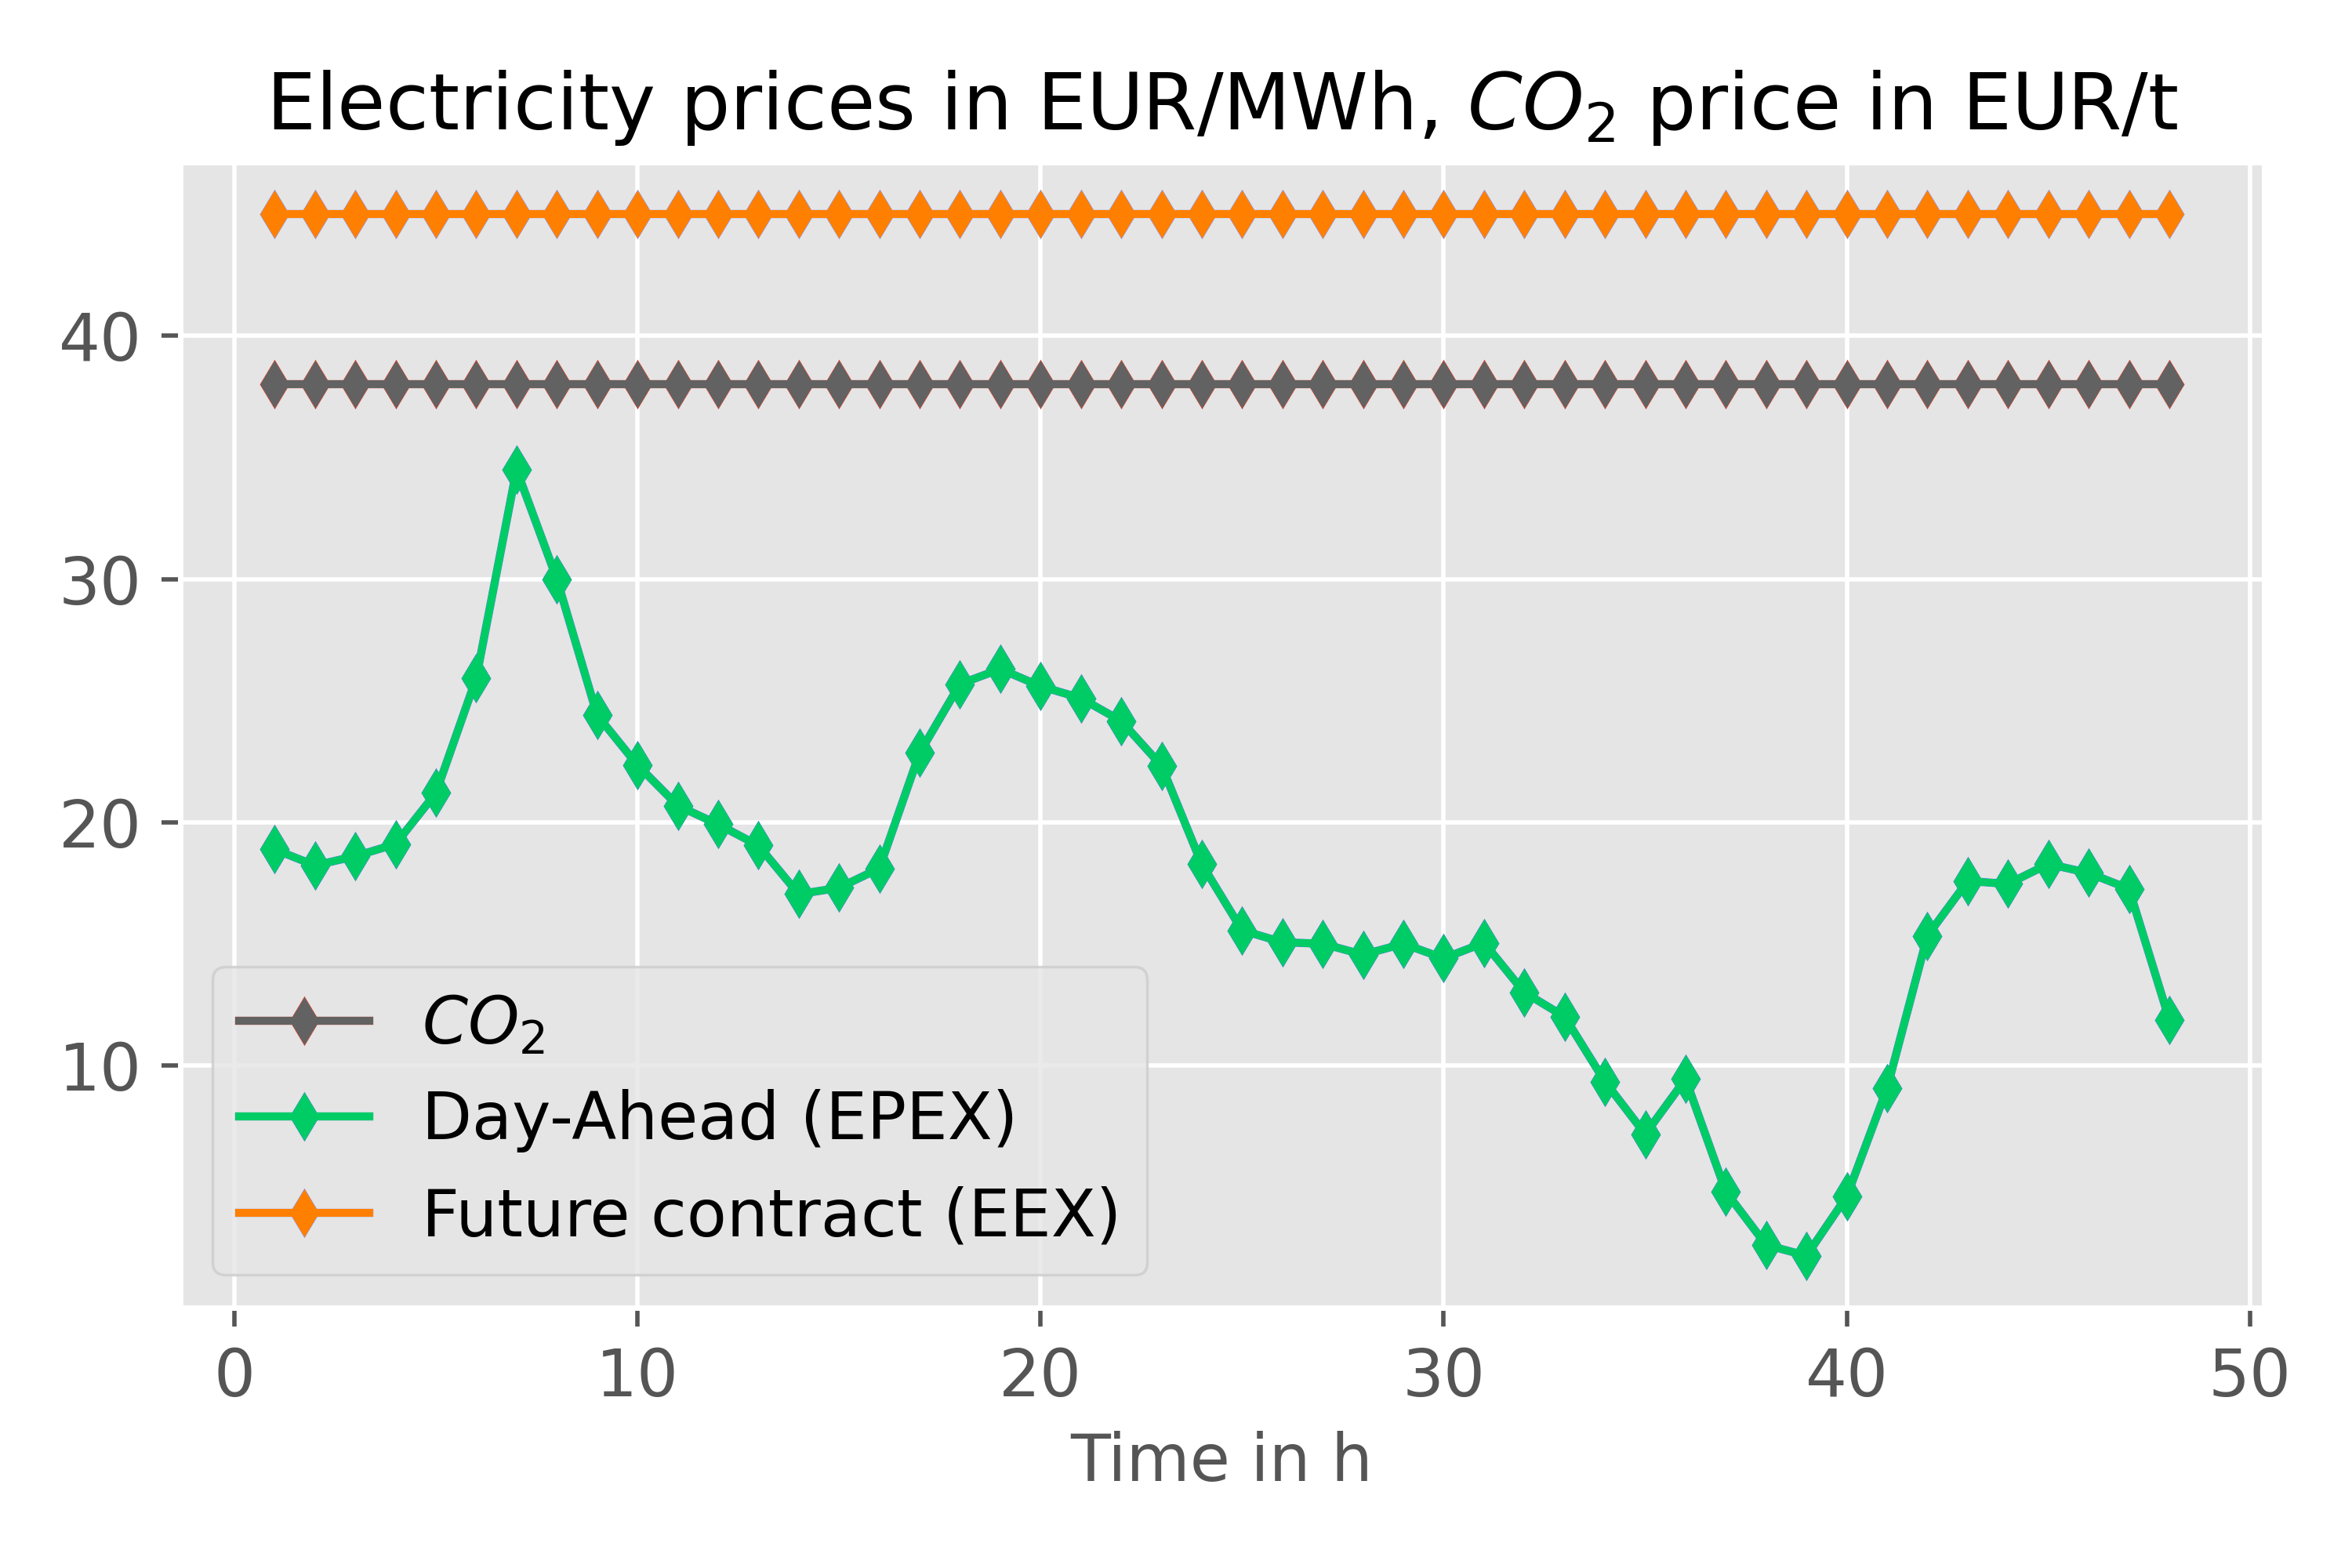
\includegraphics[width=0.75\linewidth]{figures/numerical_example_prices.png}
	\caption{Future contract (orange), CO\textsubscript{2} (gray), and day-ahead spot market (green) price}
	\label{fig:prices}
\end{figure}

\paragraph{Programming environment and open-source access} The bi-level optimization model (Equations \labelcref{bi_1} and \labelcref{bi_2}) is implemented in Python using the modeling framework Pyomo \cite{hart2017optimization} and the analysis and visualization package Pyam \cite{gidden2019pyam}.\footnote{\url{https://pyam-iamc.readthedocs.io/en/latest/}} The optimization problem is solved with the solver Gurobi version 9.0.3. Note that the open-source model and its full mathematical framework are disclosed as part of the publication at GitHub.\footnote{\url{https://github.com/sebastianzwickl}} 
\newpage
\section{Results}\label{results}
This section presents and discusses the results of the examination of the numerical example. Section \ref{res:1_tradeoffs} shows the trade-offs, resource allocation, and energy demand provision for the hydropower plant owner and the transportation firm. Section \ref{res:2_gap} highlights the economic results for both agents including the revenues, profitability gap, and shadow prices. Section \ref{res:3_CO2} shows the sensitivity analysis for varying CO\textsubscript{2} prices and Section \ref{res:4:relax} includes a relaxation of the constant hydrogen production constraint. Section \ref{res:5_time} elaborates on a decarbonization timeline of the European energy system and, subsequently, a temporal frame of profitable hydropower-based green hydrogen production.

\subsection{Trade-offs, resource allocation, and energy demand provision}\label{res:1_tradeoffs}
Figure \ref{fig_results1} presents the production and resource allocation of the hydropower plant as well as the energy demand provision of the transportation firm. Figure \ref{fig:ressources} shows the electricity generation shares of the day-ahead spot market, the future electricity contract, and hydrogen production. It is evident that in the current price setup, the constant hydropower electricity generation band is fully used for future electricity contract trading. Hence, no hydrogen is produced. The remaining hydropower electricity generation capacity is traded at the day-ahead spot market. Figure \ref{fig:provision} (top) shows the shares of the day-ahead spot market and future electricity contract in the hydropower generation profile. The energy demand provision (conventional fossil fuel) of the transportation firm is shown in Figure \ref{fig:provision} (bottom).\footnote{Note that the constant energy demand for conventional fuels is \SI{13.72}{MWh \per \hour} as the energy density factor $\beta^{con}$ must be taken into account.}

\begin{figure}[h]
	\begin{subfigure}[c]{1\textwidth}
		\centering
		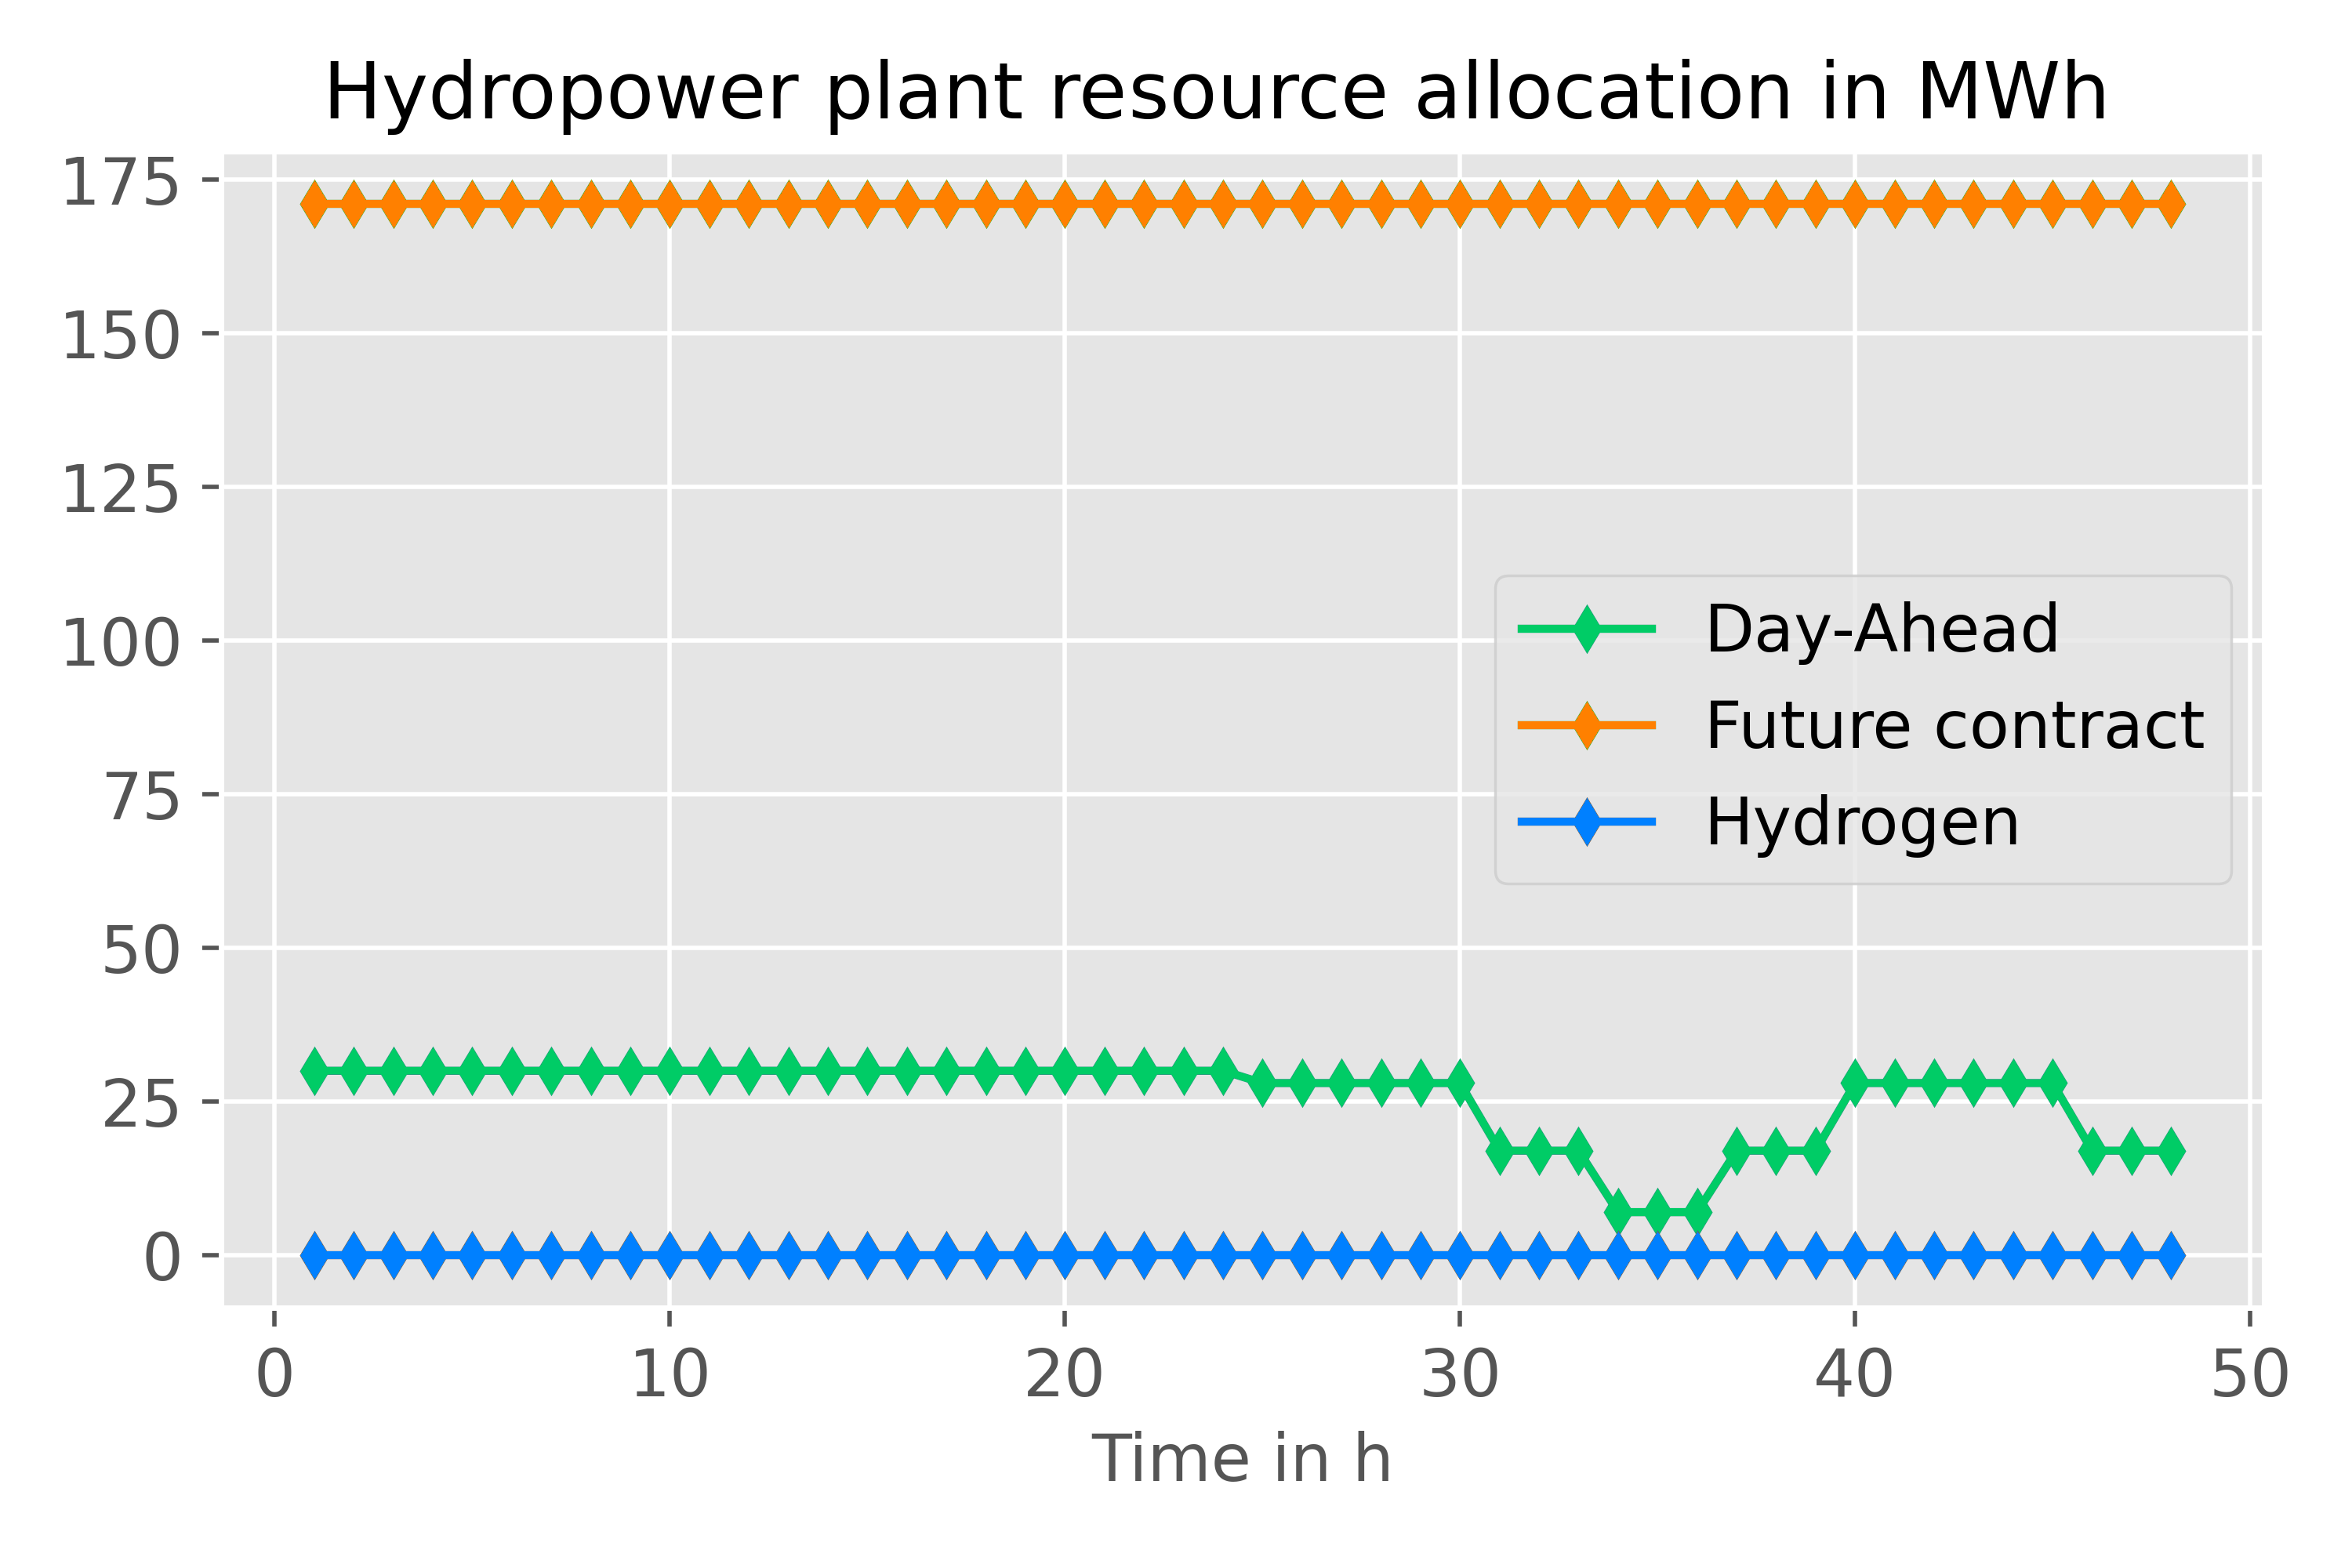
\includegraphics[width=0.8\linewidth]{figures/Ressource allocation.png}
		\subcaption{Hydropower plant resource allocation}
		\label{fig:ressources}
	\end{subfigure}
	\newline
	\newline
	
	\begin{subfigure}[c]{1\textwidth}
		\centering
		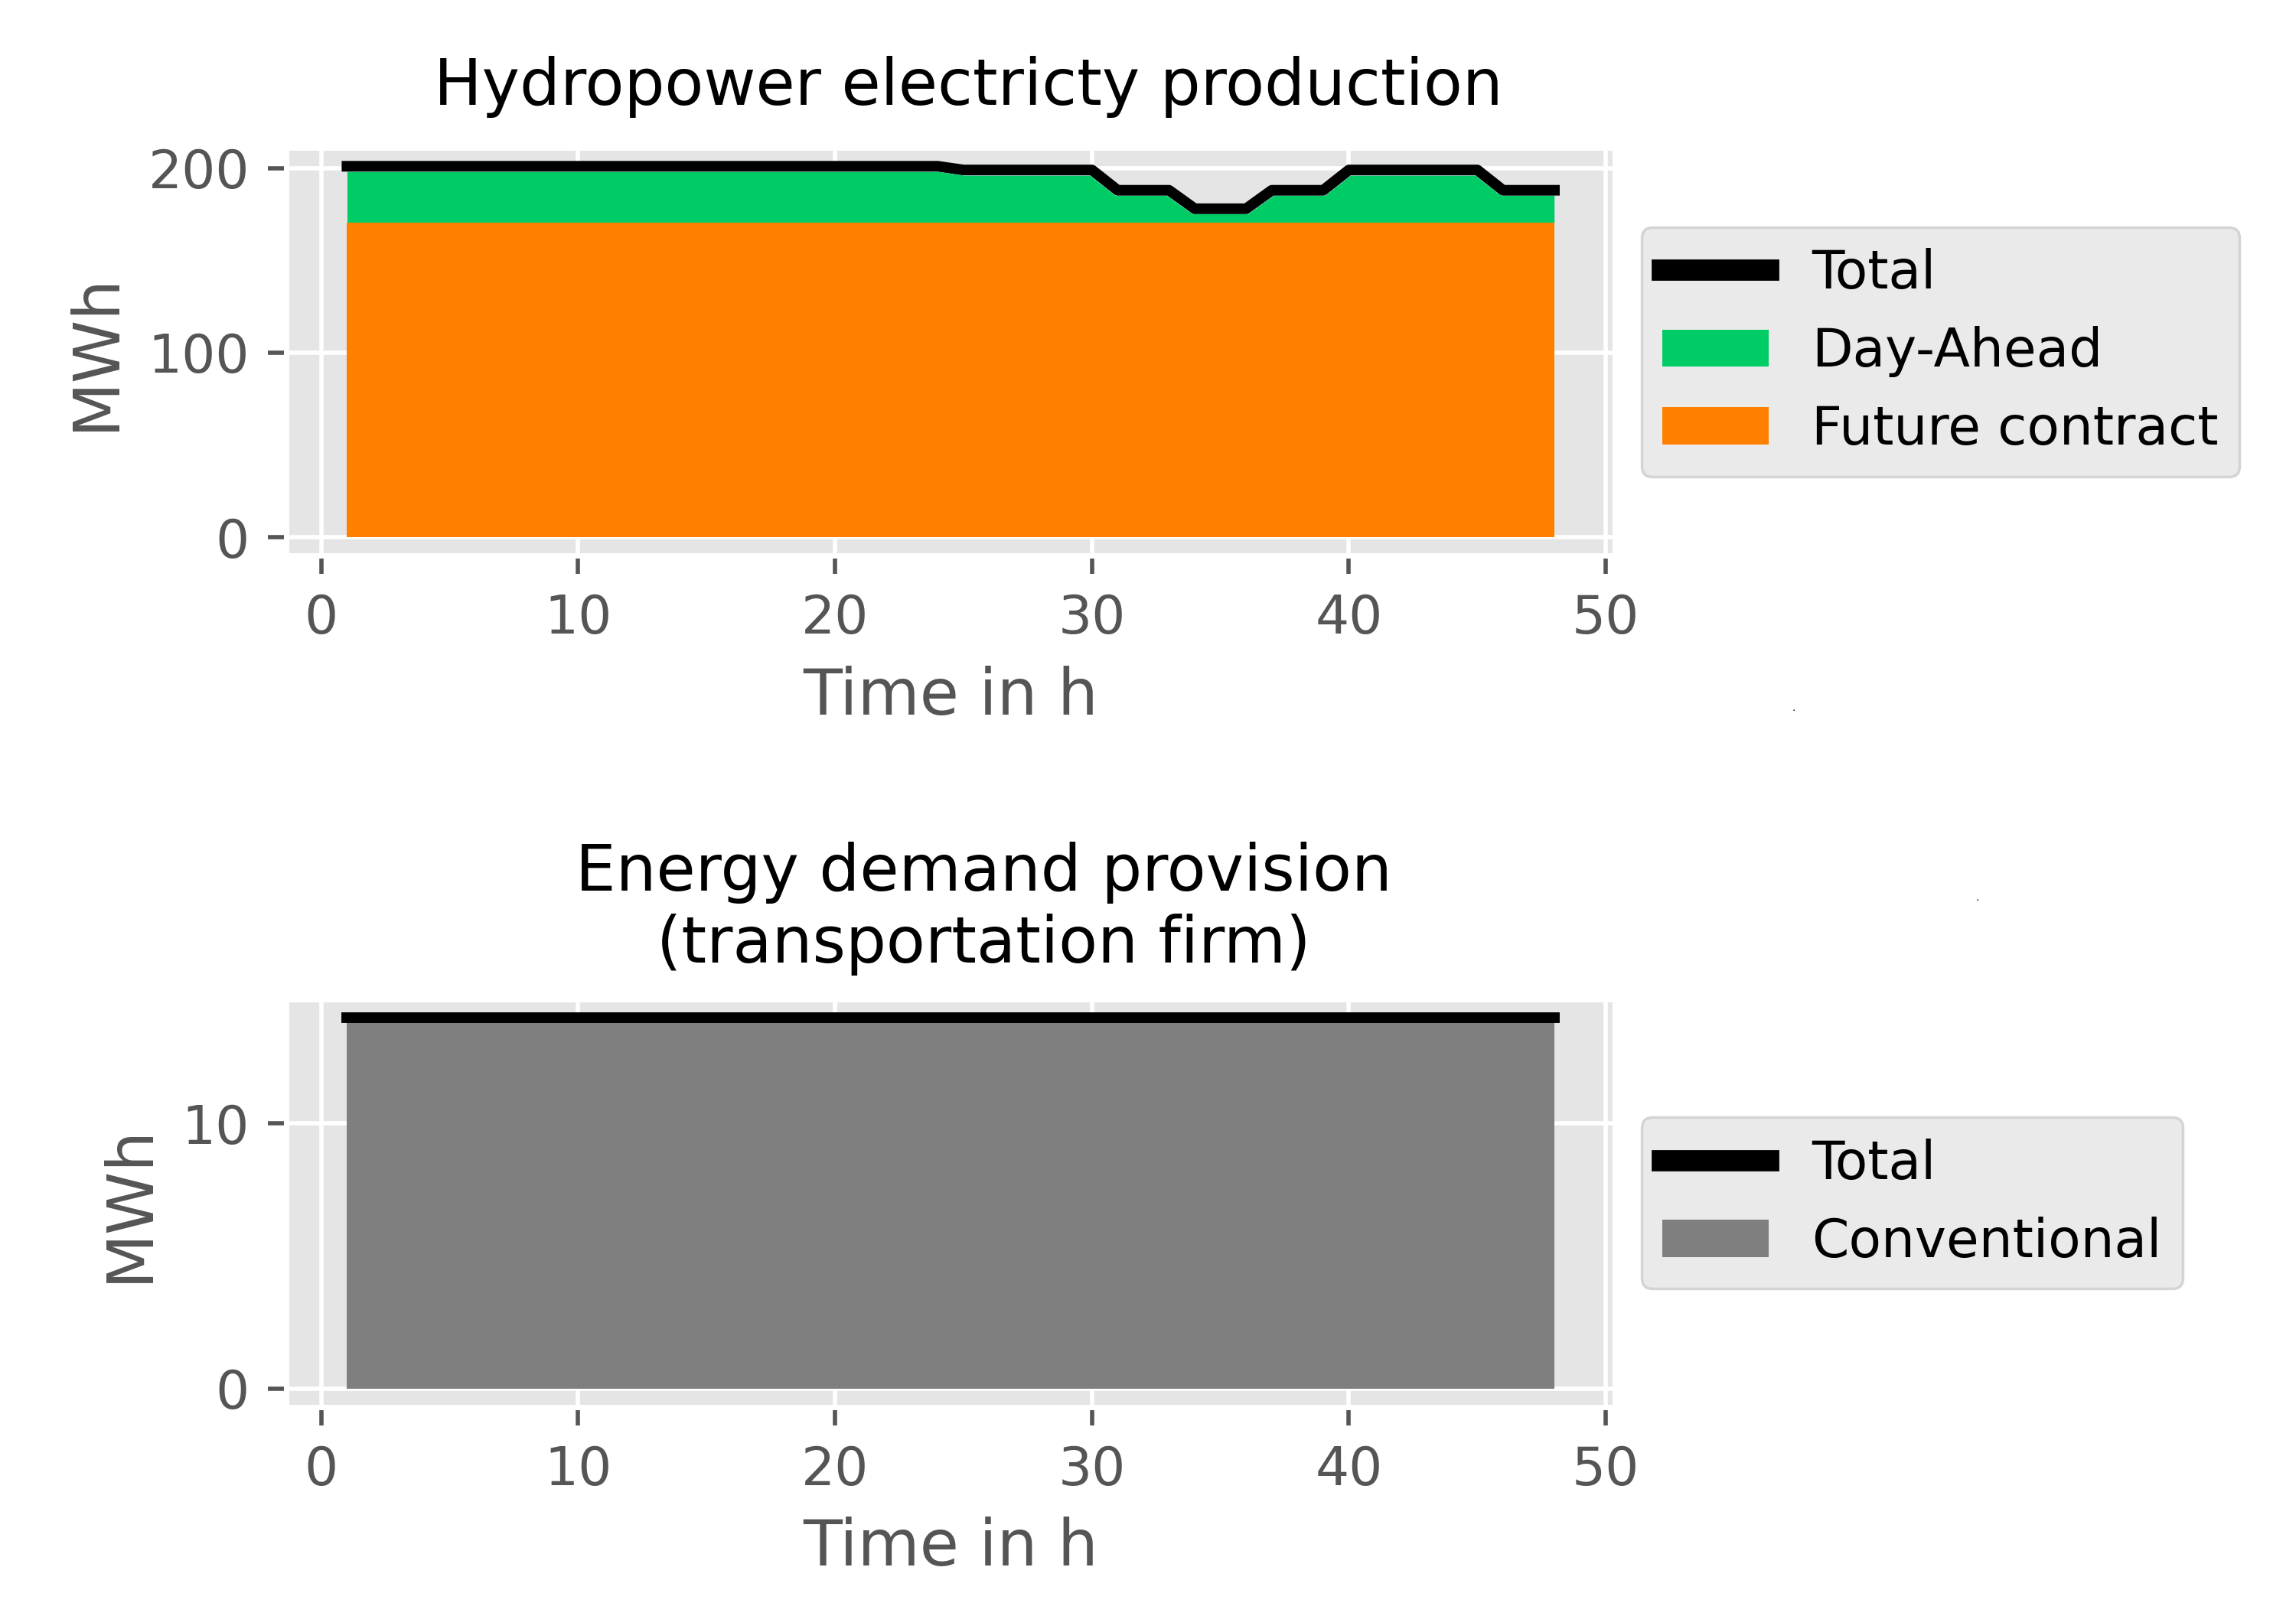
\includegraphics[width=0.8\linewidth]{figures/Energy service provision.png}
		\subcaption{Hydropower electricity production (top) and energy demand provision (bottom)}
		\label{fig:provision}
	\end{subfigure}
	\caption{Hydropower plant resource allocation, electricity production, and energy demand provision of the transportation firm}
	\label{fig_results1}
\end{figure}
\cleardoublepage
\subsection{Revenues, profitability gap and shadow price}\label{res:2_gap}
Table \ref{tab:revenues} shows the revenues of the hydropower plant owner and the corresponding amounts of electricity generated. The total revenues are \SI{391~650}{EUR}, split into \SI{94}{\%} earned from the future contract and \SI{6}{\%} from the day-ahead spot market. 

\begin{table}[h]
	\setlength{\extrarowheight}{.5em}
	\centering
	\begin{tabular}{lrr}
		\toprule
		Type & Revenues in EUR & Electricity generation in MWh \\
		\hline 
		Day-Ahead    & \SI{22~706}{} (\SI{6}{\%}) & \SI{1~230}{} (\SI{13}{\%})\\
		Future contract & \SI{368~944}{} (\SI{94}{\%})& \SI{8~208}{} (\SI{87}{\%})\\
		Hydrogen    & - & -\\
		\hline 
		Total & \SI{391~650}{} & \SI{9~438}{}\\
		\bottomrule
	\end{tabular}
	\caption{Total hydropower plant revenues/electricity generation and its components}
	\label{tab:revenues}
\end{table}

In addition, Figure \ref{fig:profit_gap} shows the resource opportunity costs of hydropower for day-ahead and future electricity contract delivery. 

\begin{figure}[h]
	\centering
	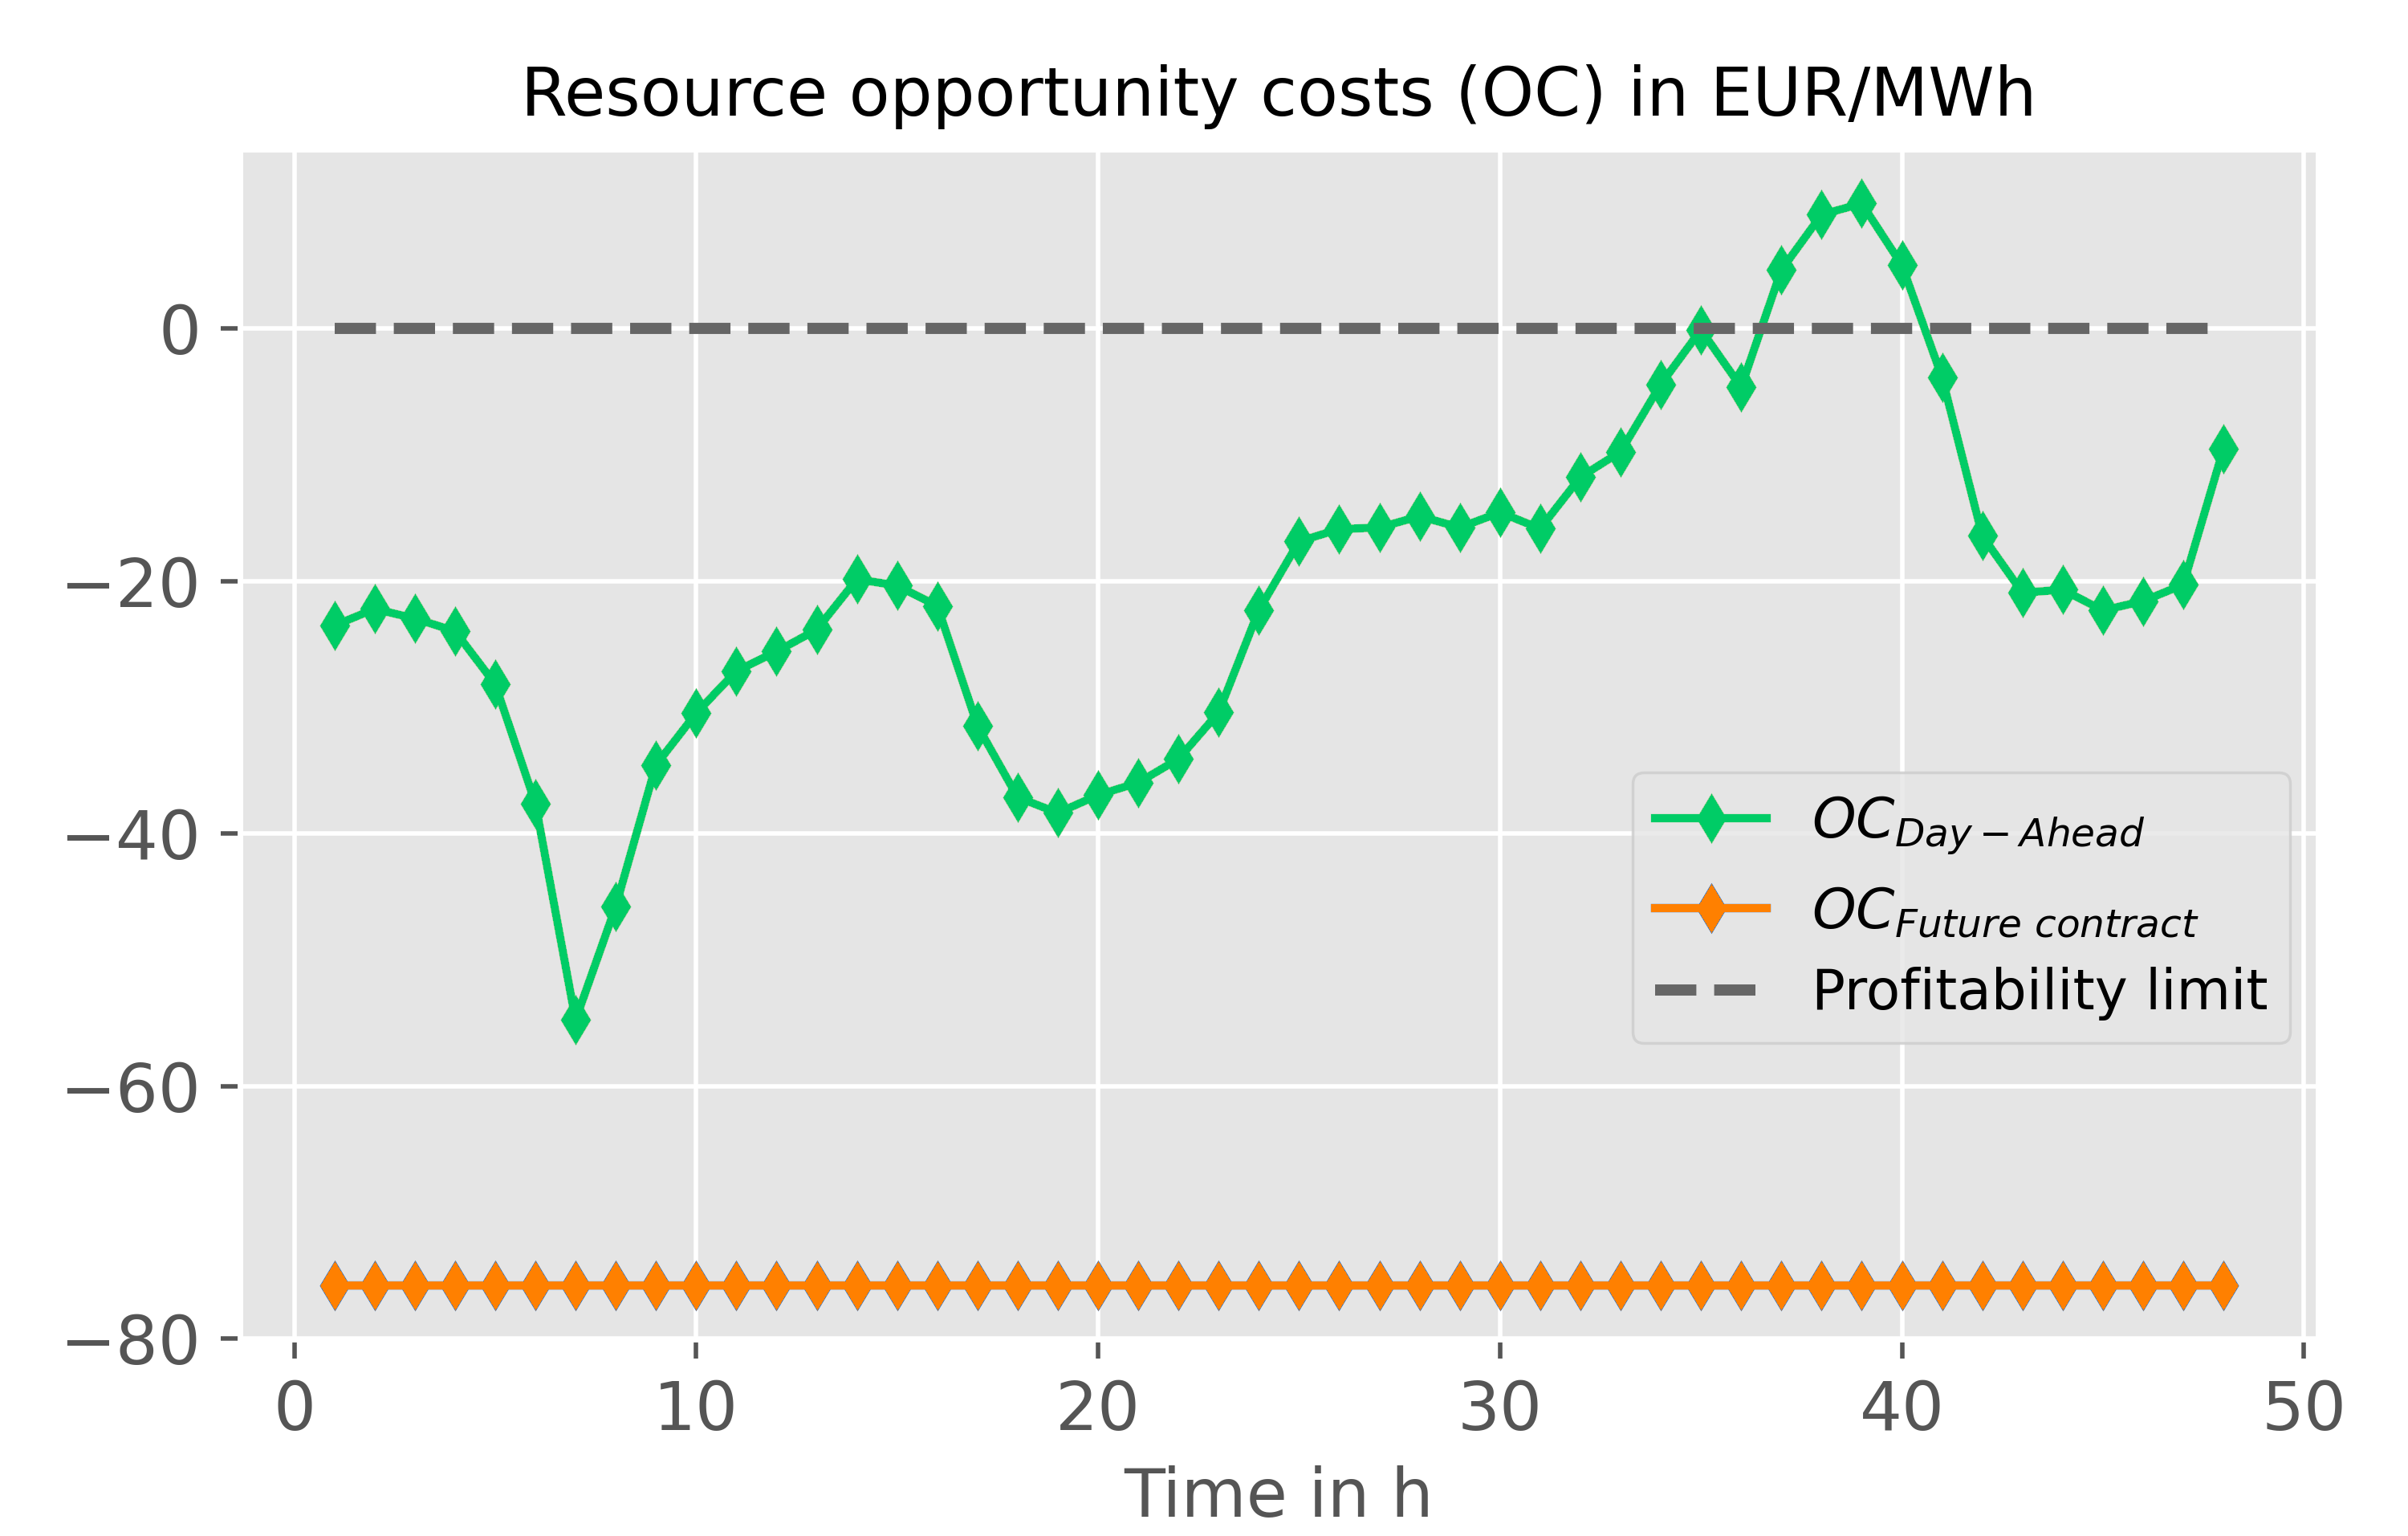
\includegraphics[width=0.9\linewidth]{figures/Profitability gap.png}
	\caption{Profitability gap for hydrogen production using the resource opportunity costs for day-ahead and future contract electricity generation}
	\label{fig:profit_gap}
\end{figure}

Hence, the profitability gap for the production of an additional hydrogen unit is indicated by the difference (gap) between the gray dashed line (profitability limit) and (i) the green line for the day-ahead, and (ii) the orange line for the future contract unit replacement for each time step $t$. The production of hydrogen through using a future contract generation unit declines total revenues of the hydropower owner by almost \SI{80}{EUR \per MWh}. Moreover, short-term production of hydrogen based on electricity generation previously traded at the day-ahead spot market is also unprofitable in most hours (see those hours where the green line is above the dashed gray one). In hours \SI{37}{} to \SI{40}{}, the green line is above the profitability limit, and green hydrogen may be produced profitably during this short period.

\subsection{Sensitivity analysis regarding CO2 pricing}\label{res:3_CO2}
In this section, the effects of increasing $CO_2$ prices on the energy prices and quantities are analyzed. Whereas the markup of a $CO_2$ price on the conventional fuel (i.e., diesel) is easily presentable, the $CO_2$ price effects on both the future electricity contract and day-ahead spot market are elusive. Therefore, the $CO_2$ price dependency is discussed on the basis of a sensitivity analysis in this section. Figure \ref{fig_results2} shows the hydrogen price set by the hydropower plant owner. This price depends on (i) the $H_2$ producer's (hydropower plant owner) opportunity costs and (ii) the $H_2$ consumer's (transportation firm) shadow price (see Figure \ref{fig:price}). The hydropower plant revenues including its components are shown in Figure \ref{fig:revenues}. Note that the results take into account the fact that the hydropower plant owner (leader) has full information about the follower's (transportation firm) shadow price. On the basis of the price settings used in the analysis in this work so far, the opportunity costs for hydrogen production are \SI{90}{EUR \per MWh} and include both the hydrogen production efficiency and the future electricity contract price. 

\begin{figure}[h]
	\begin{subfigure}[c]{1\textwidth}
		\centering
		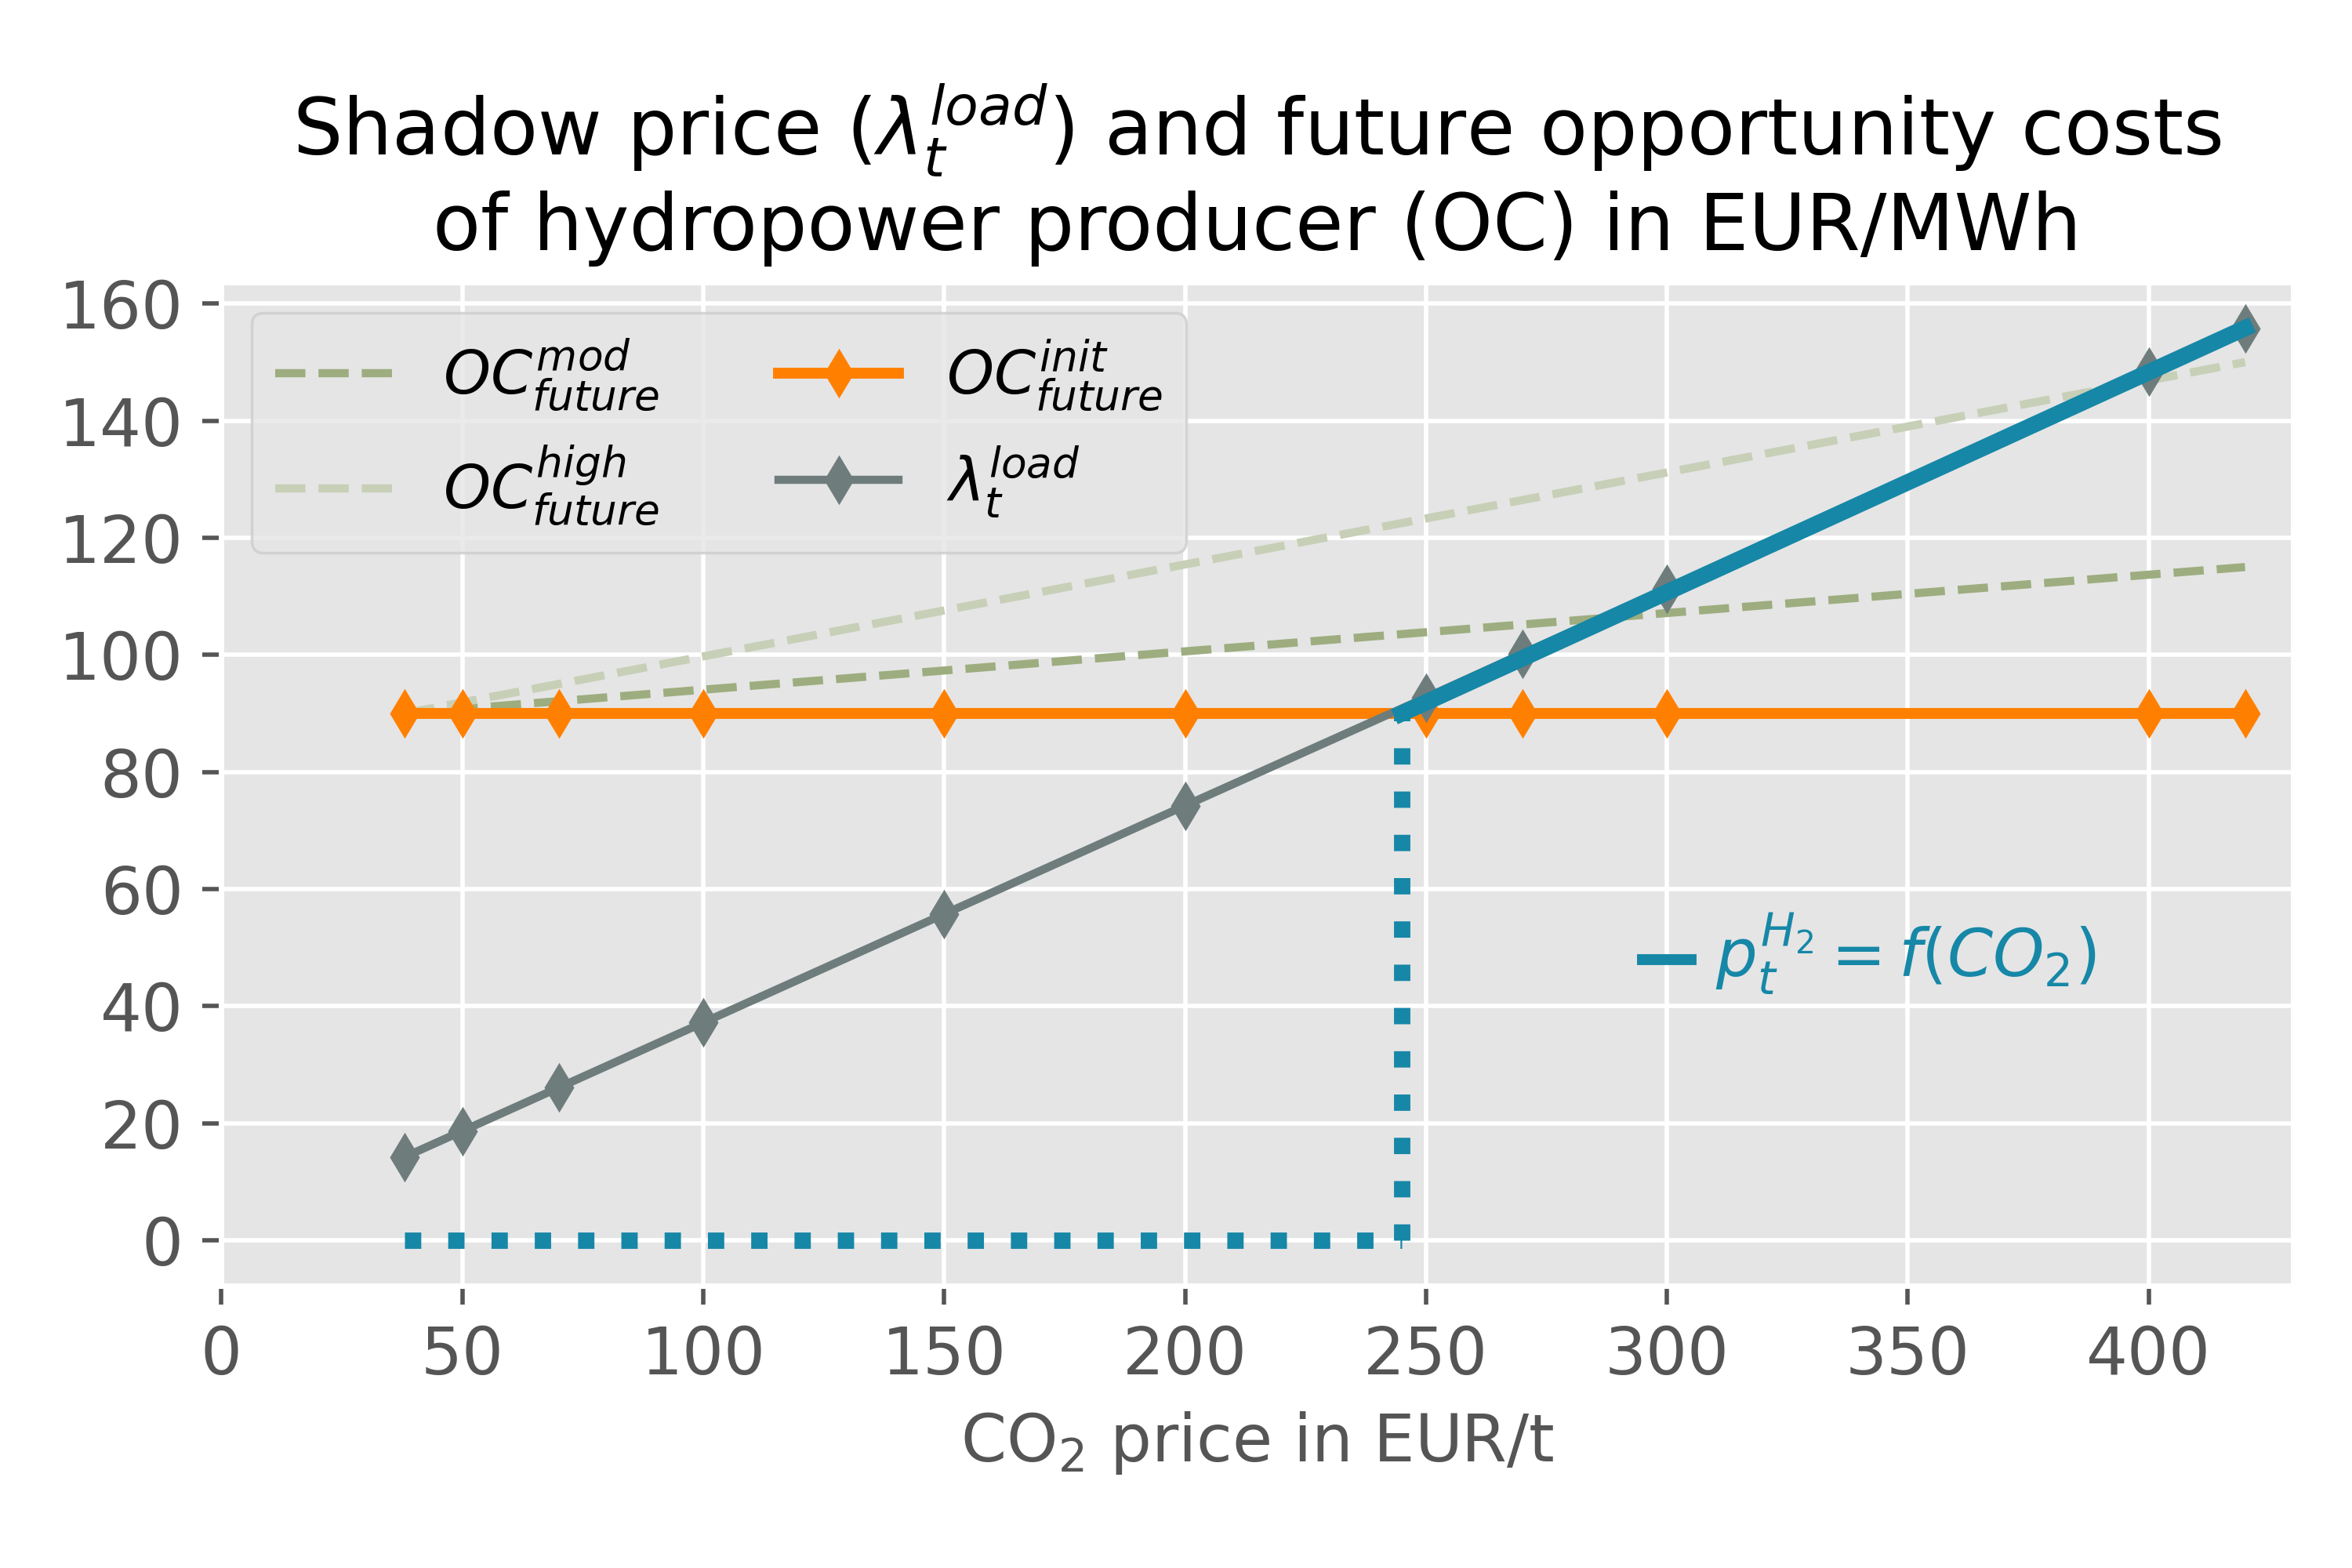
\includegraphics[width=0.8\linewidth]{figures/Break even.png}
		\subcaption{$p_{t}^{H_2}$ set depending on shadow price and opportunity costs}
		\label{fig:price}
	\end{subfigure}
	\newline
	\newline
	
	\begin{subfigure}[c]{\textwidth}
		\centering
		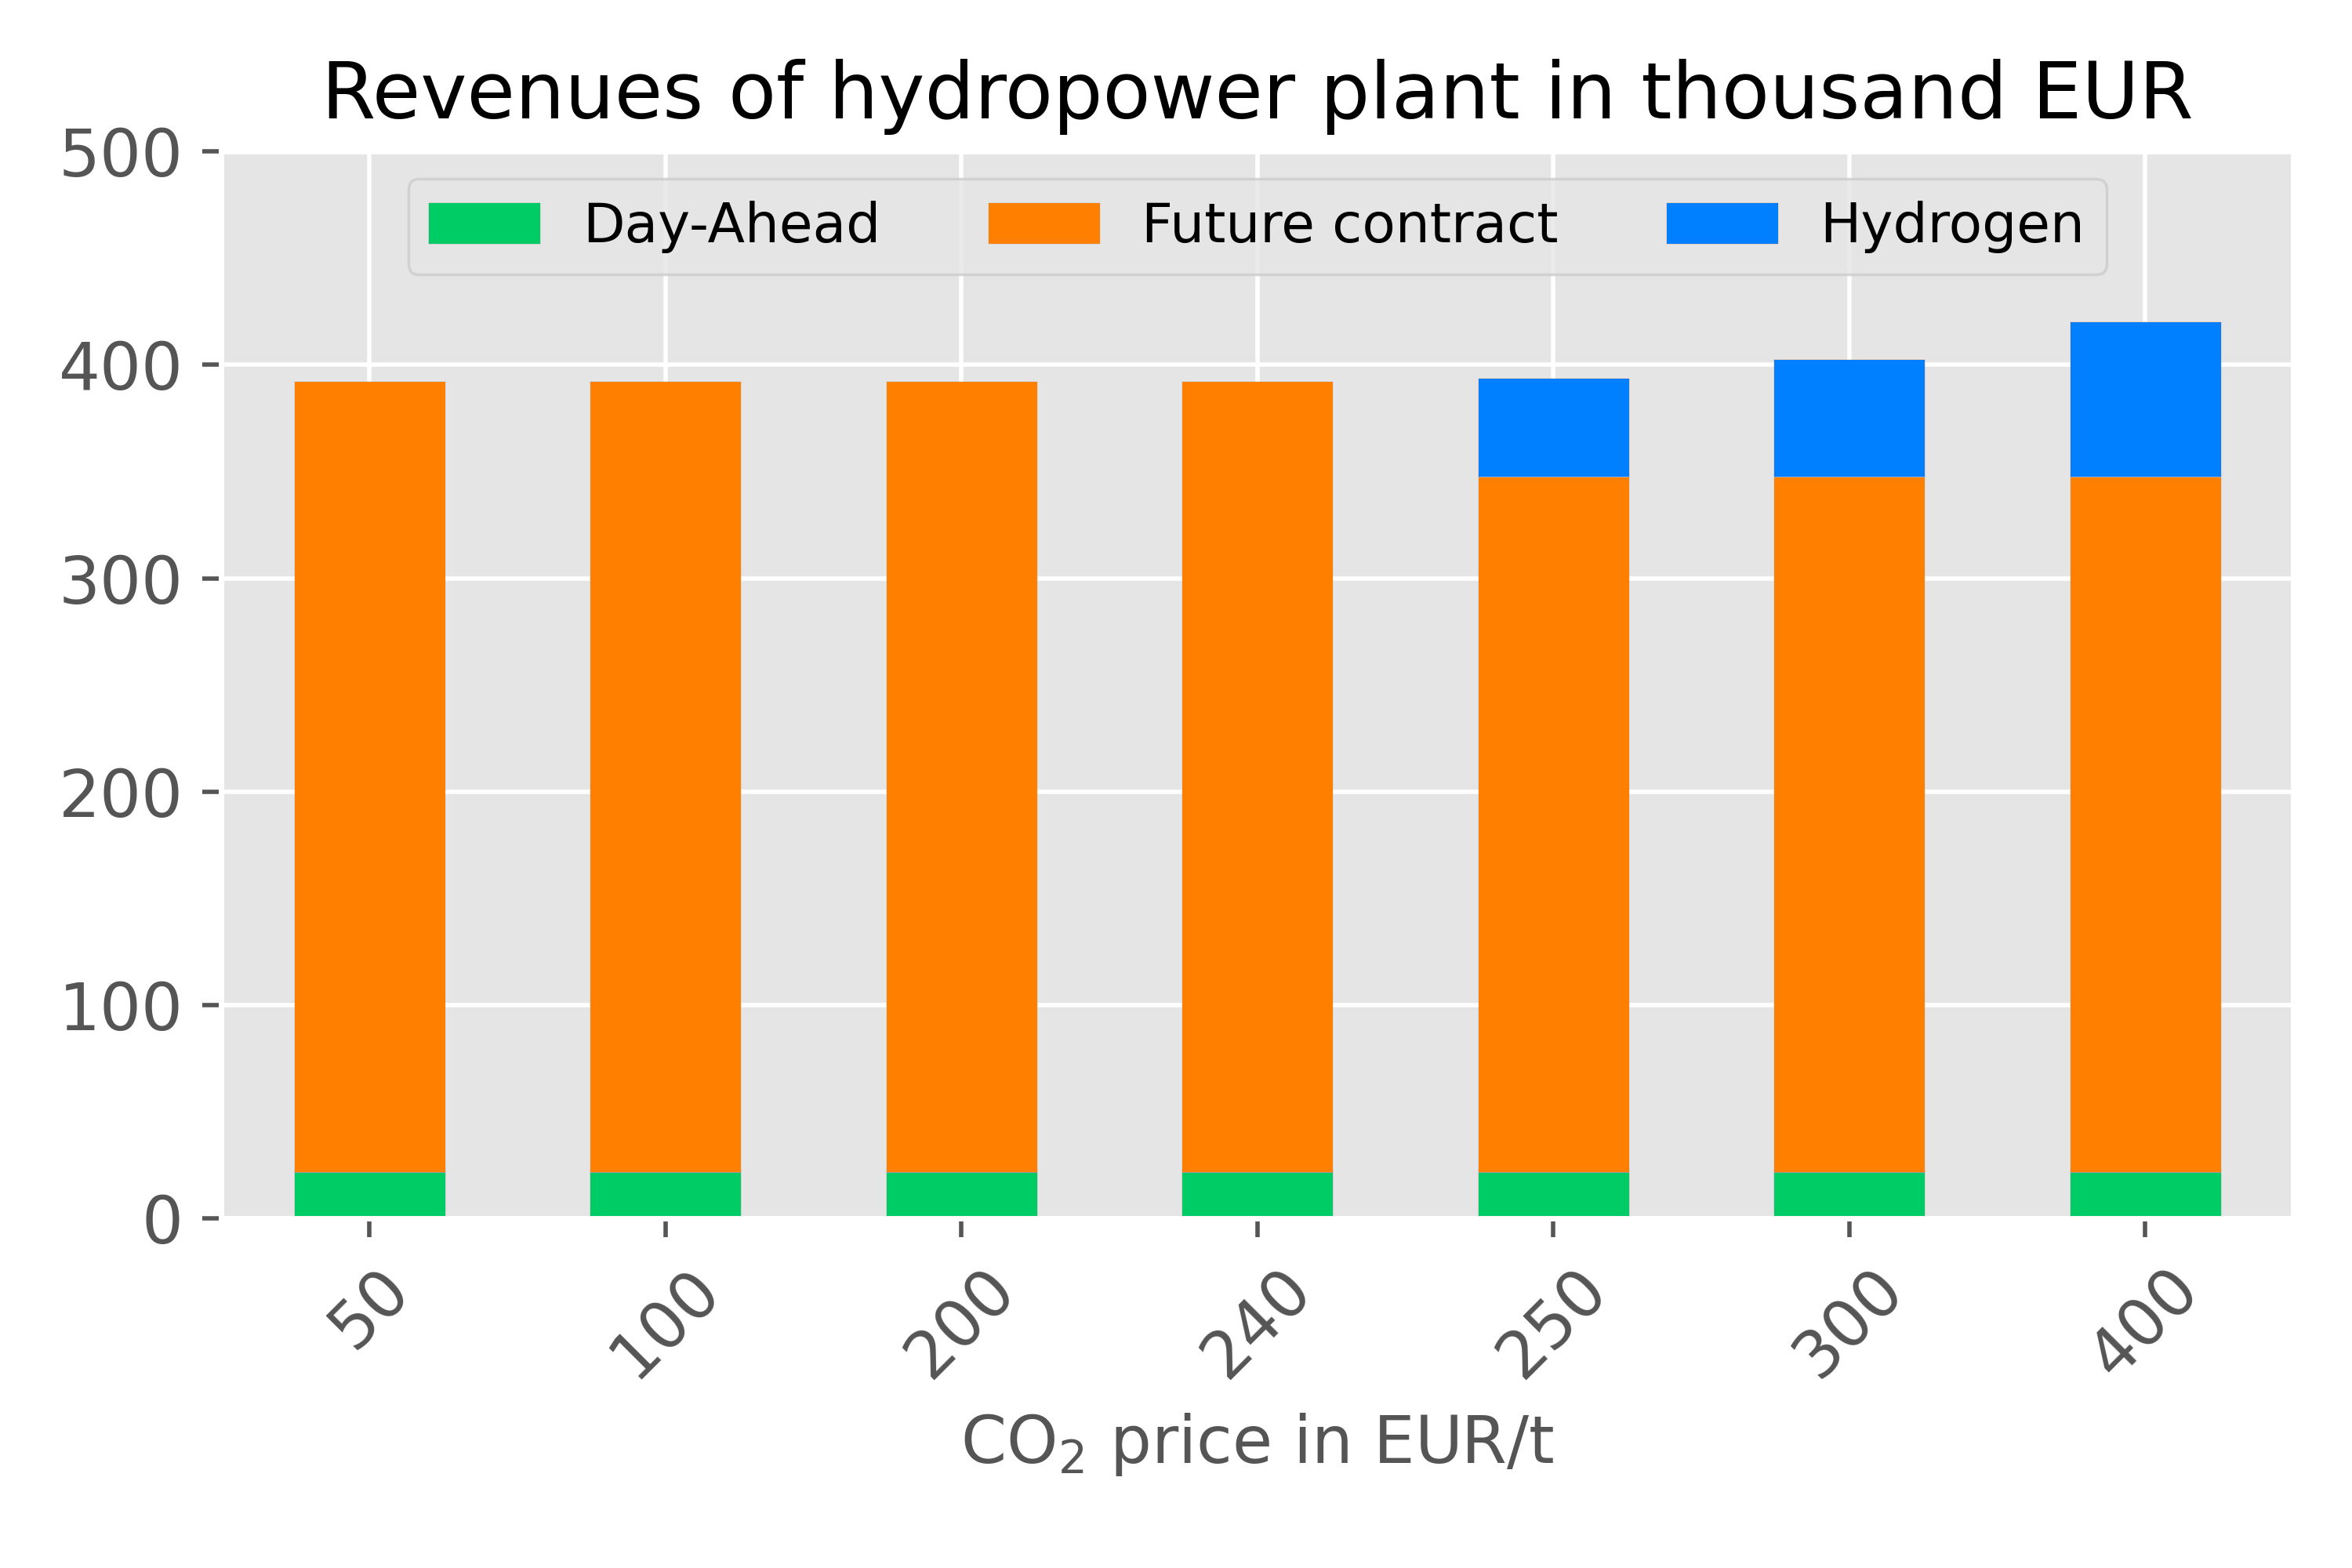
\includegraphics[width=0.8\linewidth]{figures/Revenues.png}
		\subcaption{Hydropower revenues and its components}
		\label{fig:revenues}
	\end{subfigure}
	\caption{(a) Hydrogen price ($p_{t}^{H_2}$) depending on the shadow price ($\lambda_{t}^{load}$) and its opportunity costs (OC) for different $CO_2$ prices, (b) revenues (including components) for the same scale of varying $CO_2$ prices}
	\label{fig_results2}
\end{figure}
\cleardoublepage
Up to a $CO_2$ price of almost \SI{245}{EUR \per t}, no hydrogen price $p_t^{H_2}$ is set as the leader's decision (opportunity costs $\leq$ revenues). This is indicated by the dashed blue line in Figure \ref{fig:price}. At the intersection point in Figure \ref{fig:price}, $p_t^{H_2}$ is set by the leader in order to maximize its revenues accordingly. The revenues of the hydropower plant owner are shown in Figure \ref{fig:revenues}. Note that the intersection point significantly depends on the future electricity contract price. For increasing future electricity contract prices an intersection point (i.e., $p_t^{H_2}$) is achieved at higher $CO_2$ prices only. This is qualitatively indicated by the two dashed green lines in Figure \ref{fig:price}. Hence, Figure \ref{fig:contour} shows the required $CO_2$ price levels replacing conventional fuels of the transportation firm by hydrogen, taking into account both a variation (increase) of the future electricity contract price and hydrogen production efficiency. 

\begin{figure}[h]
	\centering
	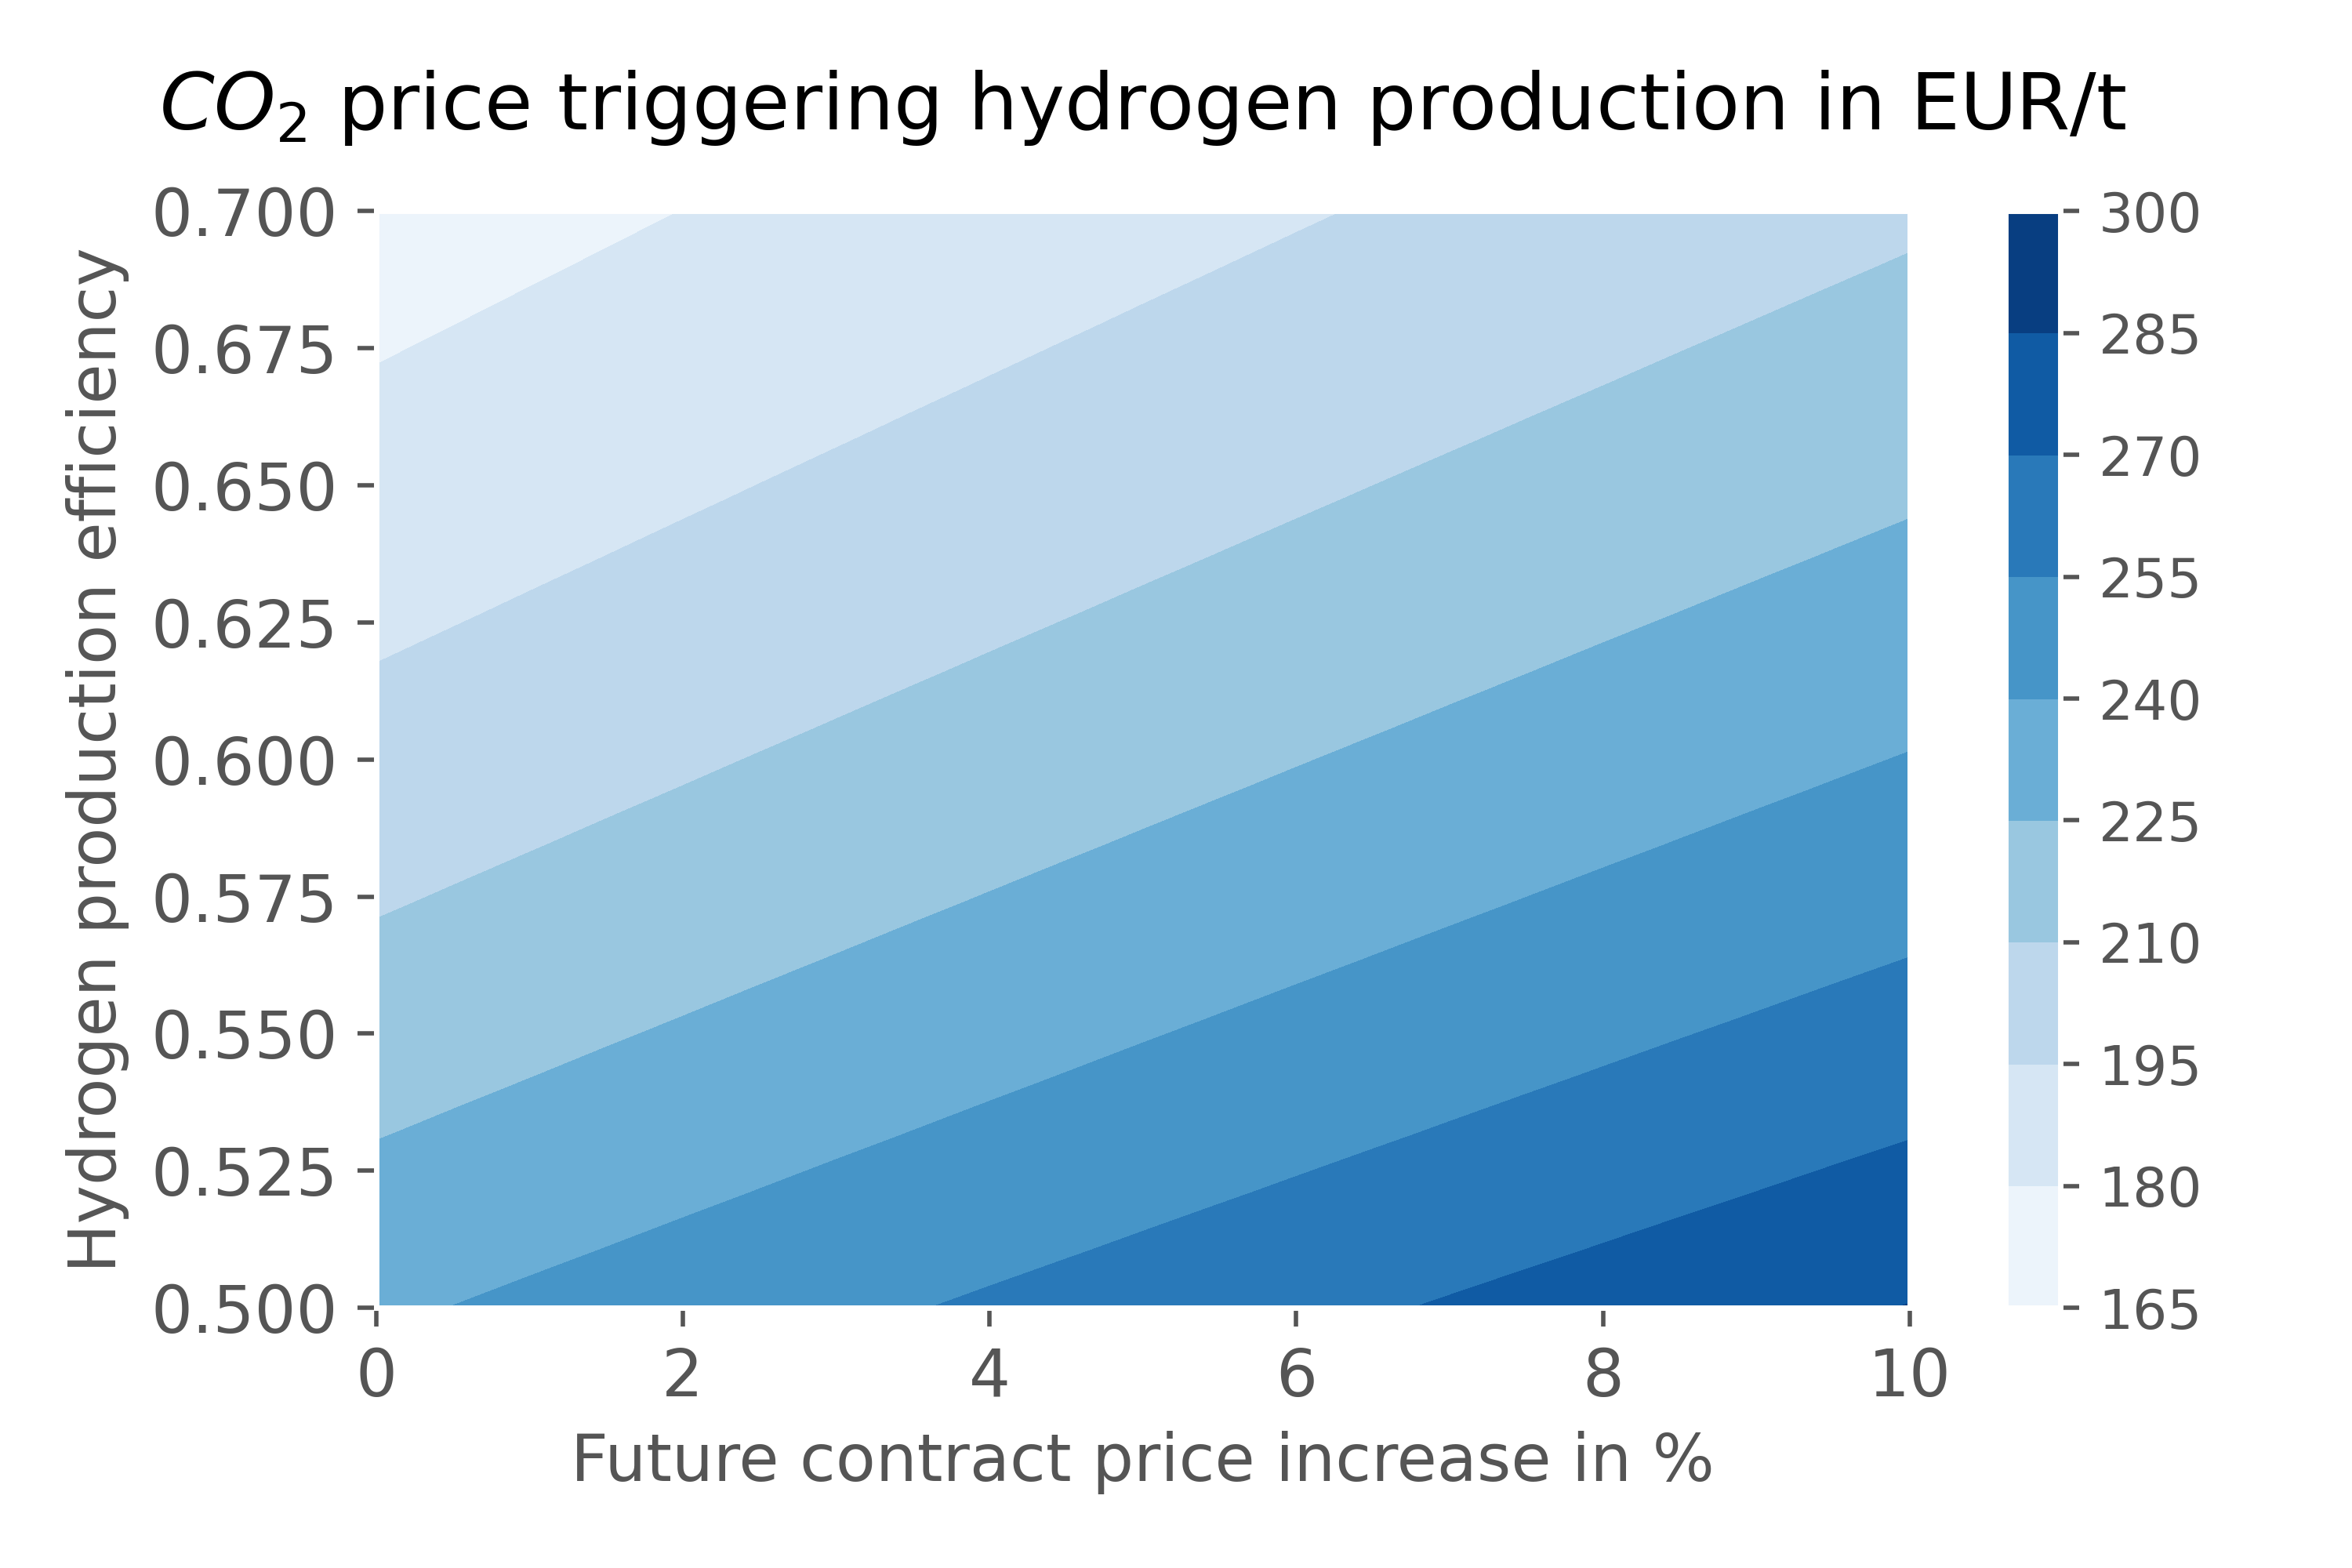
\includegraphics[width=0.8\linewidth]{figures/Contour.png}
	\caption{Calculated $CO_2$ prices (y-axis, right) triggering the penetration of hydrogen in vehicle fleet supply of the transportation firm depending on future electricity contract price increase (x-axis) and hydrogen production efficiency (y-axis, left)}
	\label{fig:contour}
\end{figure}

An increasing future electricity contract price expects higher $CO_2$ prices, triggering green hydrogen supply of the transportation firm's vehicle fleet. Note that the intersection point from Figure \ref{fig:price} (crossover from the dashed to solid blue line) is located in the origin of the coordinates. In the sensitivity analysis of an increase of the future electricity contract price by \SI{10}{\%} affected by a rising $CO_2$ price, the calculated required $CO_2$ price is \SI{300}{EUR \per t}. In terms of hydrogen production efficiency, a higher efficiency naturally expects a lower required $CO_2$ price to trigger profitable green hydrogen production. 

\subsection{Constant hydrogen production relaxation}\label{res:4:relax}
In the following sensitivity analysis, a constraint of the modeling framework is relaxed to enable more flexible hydrogen production. In particular, the bi-level optimization problem (Equations \labelcref{bi_1} and \labelcref{bi_2}) is relaxed by the constraints in Equations \labelcref{L5} and \labelcref{L7}. This enables the hydropower plant owner to have a more flexible production of hydrogen by unlocking the initial exclusive day-ahead spot market delivery in addition to the still possible future electricity contract trade-offs. Therefore, no constant hydrogen production is obligatory anymore. If there is a clear price signal instead, hydrogen is produced variably. Note that this also takes into account a more adjustable and flexible hydrogen consumer. Moreover, it may be assumed that the produced hydrogen can be traded with various hydrogen consumers (exemplarily in the transportation sector), which provides a certain flexibility over time.\vspace{0.3cm}

According to the empirical assumptions used in the numerical example above, the full-load hours of hydrogen production are \SI{156}{\hour} for a current $CO_2$ price of \SI{38}{EUR \per \tonne}. The hydrogen production utilization indicator significantly depends on the development/increase of the energy (mainly day-ahead spot market) and $CO_2$ prices. Therefore, Figure \ref{fig:full_load} examines the achievable full-load production hours, taking into account different energy price developments affected by rising $CO_2$ prices. In the case that the day-ahead spot market price remains unchanged and the $CO_2$ price increases, (a) shows the development of the full-load hours. Accordingly, (b)-(d) show the full-load hours for an average increase of the day-ahead spot market of (b) \SI{0.05}{EUR \per MWh}, (c) \SI{0.125}{EUR \per MWh}, and (d) \SI{0.25}{EUR \per MWh}  per increase of the $CO_2$ price by \SI{1}{EUR \per \tonne}. The results show that the increase in the day-ahead spot market price limits the full-load hours (the higher the increase, the lower the full-load hours). Note that the different day-ahead spot market price developments could be interpreted as different electricity generation technology mixes, and hence renewable energy technology penetration rates.\footnote{In this context, see also related assumptions in \cite{breitschopf2016prices} and \cite{fina2019profitability}. Note that this work's increase of the day-ahead spot market price affected by rising $CO_2$ prices is more conservative in comparison. This means that the increase of the day-ahead price is lower than the referenced studies. The reason for this is that the results in Figure \ref{fig:full_load} indicate already almost no profitable green hydrogen production at a certain wholesale electricity price level.}

\begin{figure}[h]
	\centering
	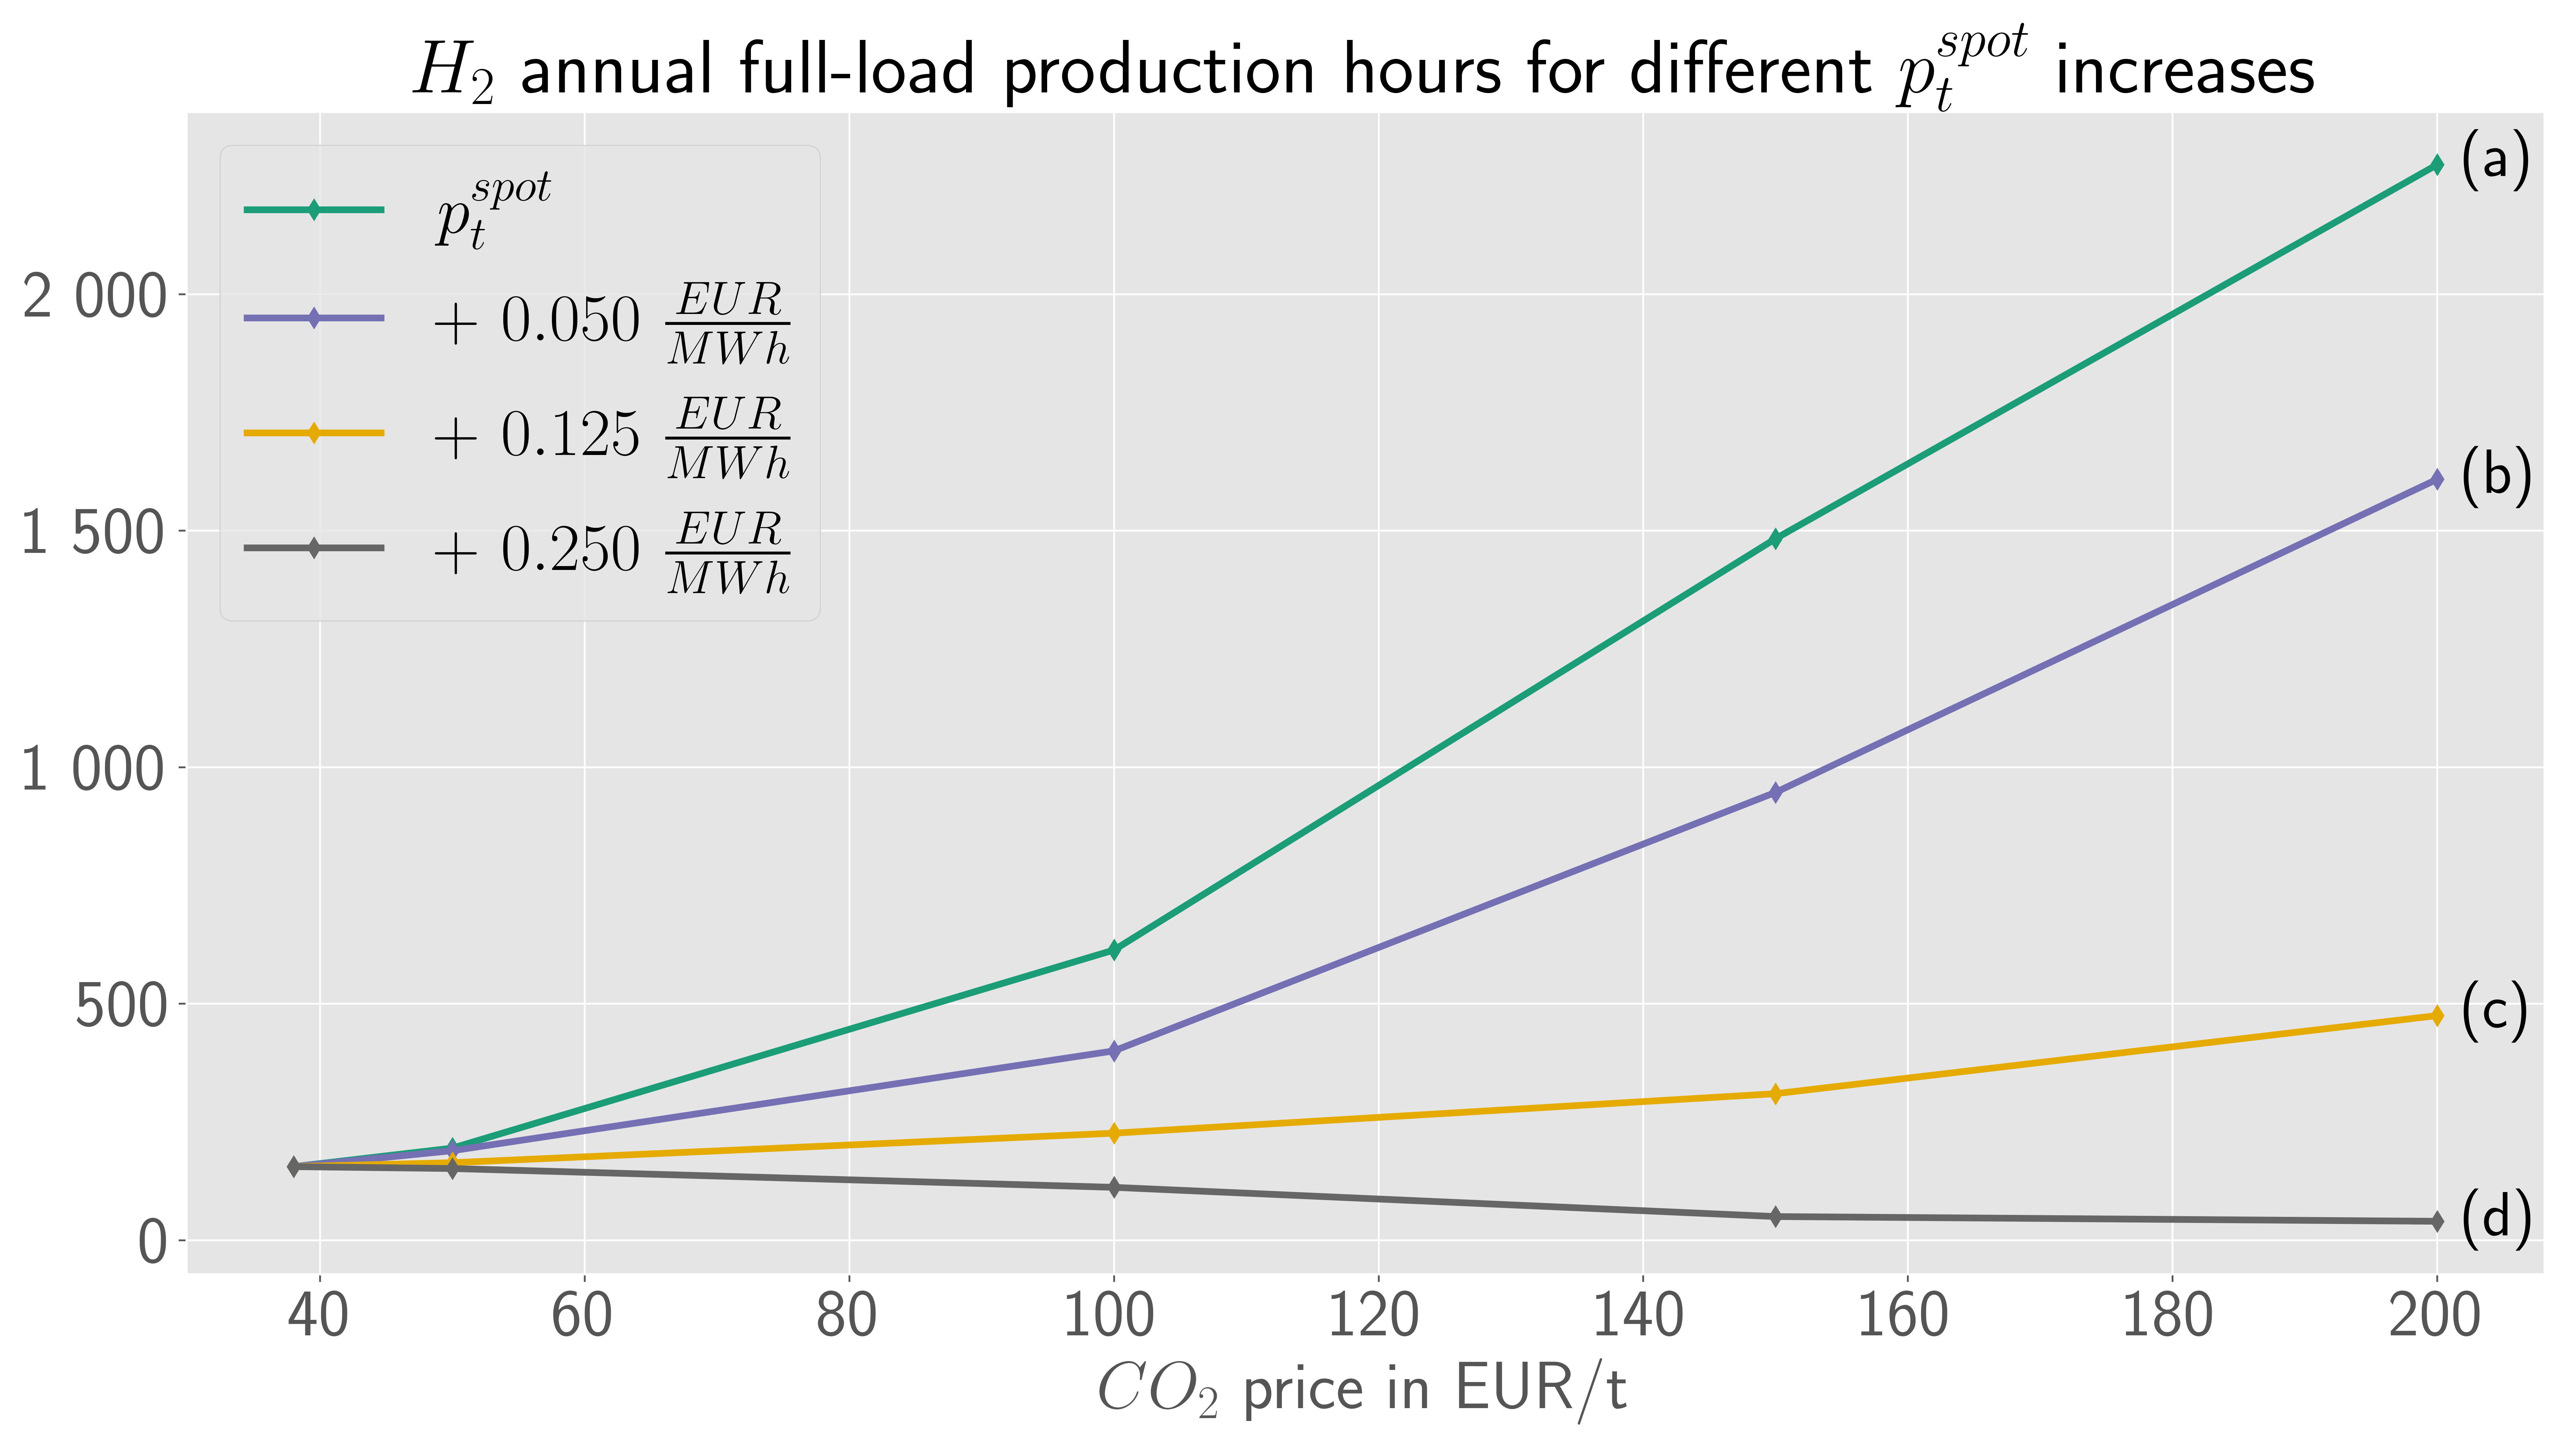
\includegraphics[width=0.9\linewidth]{figures/utilization_v0.1.png}
	\caption{$H_2$ annual full-load hydrogen production hours for varying $CO_2$ prices and different average day-ahead spot market price ($q_{t}^{spot}$) increases per increase in the $CO_2$ price: $q_{t}^{spot}$ (green), $q_{t}^{spot} + \SI{0.05}{\frac{EUR}{MWh}}$ (purple), $q_{t}^{spot} + \SI{0.125}{\frac{EUR}{MWh}}$ (orange), and $q_{t}^{spot} + \SI{0.25}{\frac{EUR}{MWh}}$ (gray)} 
	\label{fig:full_load}
\end{figure}

\subsection{Energy system decarbonization timeline and temporal frame}\label{res:5_time}
In this section, the calculated $CO_2$ price levels/ranges for profitable green hydrogen production are matched with outlined $CO_2$ prices in recent European energy system scenario studies that take into account the European decarbonization needs up to 2050 for complying to the ambitious \SI{1.5}{\degreeCelsius} climate targets. This enables the estimation of a rough temporal frame when green hydrogen production from hydropower is expected to be profitable and reaches viability as a self-sustaining business case.\vspace{0.3cm}

For this reason, the four different quantitative decarbonization scenario studies from the research project {openENTRANCE} (\url{https://openentrance.eu/}) are used for the comparison. The four scenarios as well as the corresponding $CO_2$ prices governing European energy system decarbonization are comprehensively described in \cite{auer2020development, auer2020quantitative}. The underlying storylines outlining the narrative frames of the quantitative scenarios can be found in \cite{auer2019quantitative}. The four storylines are called as follows: \textit{Gradual Development}, \textit{Directed Transition}, \textit{Societal Commitment}, and \textit{Techno-Friendly}. They describe possible future developments of a low-carbon European energy system taking into account different key drivers and a variety of future uncertainties. The latter three storylines aim for meeting the ambitious \SI{1.5}{\degreeCelsius} global warming target, whereby the remaining one (\textit{Gradual Development}) approaches the less ambitious \SI{2.0}{\degreeCelsius}. For a detailed description of the storylines, see references \cite{auer2020development, auer2020quantitative}.\vspace{0.3cm}

Storytelling about a possible future European energy world moves in a three-dimensional space spanned by the following uncertain parameters: technology, policy, and society. Each of the three ambitious \SI{1.5}{\degreeCelsius} stories has two of the dimensions pronounced; the third dimension does not play a major role. \textit{Techno-Friendly}, for example, describes a significant market-driven technological breakthrough of new technologies that are also approved by society. Therefore, no strong energy policy interventions are necessary. On the other hand, \textit{Directed Transition}, for example, means a breakthrough of new clean technologies will only occur through strong policy incentives as the markets do not push this strongly enough and society is also too passive toward it. Eventually, \textit{Societal Commitment} describes a possible new decentralized and participatory energy world with strong societal acceptance of energy transition, driven by policy incentives of currently existing technologies, as no fundamental breakthroughs of new clean technologies are in sight. Finally, \textit{Gradual Development} is a very conservative expression of all three dimensions (a little bit of all) against the background of the \SI{2.0}{\degreeCelsius} target. Against this background, hydrogen deployment up to 2050 is different in the different scenarios in terms of both timing/quantity of market penetration and preferred sector of application. A matching of the scenario results in the {openENTRANCE} project (notably the $CO_2$ price development) with the key findings of this work is presented in Table \ref{tab:scenarios} and can be explained and summarized as follows: The $CO_2$ price range of \SI{245}{} to \SI{300}{EUR \per \tonne} (depending on key technical and economic parameter developments) identified in this work for a profitable green hydrogen business case from hydropower corresponds to the different $CO_2$ price ranges and time frames identified for hydrogen market penetration in the {openENTRANCE} project as presented in Table \ref{tab:scenarios}. This comparative analysis enables the estimation of a future timeline when the business case presented in this work could become attractive. Exemplarily, a strong policy incentivized future development (\textit{Directed Transition}) could realize the business case (in Europe) already in the period 2025-2030. On the contrary, less ambitious European decarbonization efforts (\textit{Gradual Development}) trigger the business case only after 2040. For completeness, it is important to note that the $CO_2$ price developments in the {openENTRANCE} scenario studies are not set arbitrarily but represent endogenous modeling results of the optimization problem (i.e., dual variable of the $CO_2$ budget constraint in the underlying modeling framework \cite{burandt2018genesys}). 

\begin{table}[h]
	\centering
	\setlength{\extrarowheight}{.5em}
	\scalebox{0.85}{
	\begin{tabular}{lccc}
		\toprule
		openENTRANCE scenario & Time frame&$CO_2$ prices in \SI{}{EUR \per \tonne}&Climate target in \SI{}{\degreeCelsius}\\
		\hline 
		\textit{Directed Transition} & $2025-2030$&\SI{196}{}-\SI{348}{}&\SI{1.5}{\degreeCelsius}\\
		\textit{Societal Commitment} &$2030-2035$&\SI{137}{}-\SI{273}{}&\SI{1.5}{\degreeCelsius}\\
		\textit{Techno-Friendly} & $2035-2040$&\SI{193}{}-\SI{351}{}&\SI{1.5}{\degreeCelsius}\\
		\textit{Gradual Development} & $2040-2045$&\SI{261}{}-\SI{348}{}&\SI{2.0}{\degreeCelsius}\\
		\bottomrule
	\end{tabular}}
	\caption{Time frame of hydrogen penetration and corresponding $CO_2$ price range for the four different European decarbonization scenarios (including their climate target) according to the {openENTRANCE} project}
	\label{tab:scenarios}
\end{table}





%comprehensive works in \cite{auer2020development, auer2020quantitative, auer2019quantitative}. One of the key emerging findings of his work is that a $CO_2$ price of \SI{245}{EUR \per t} to \SI{300}{EUR \per t} (depending on key technical and economic parameter developments) is required for a profitable green hydrogen business case from hydropower. This calculated $CO_2$ price is achieved by different time periods in the storylines. Table \ref{tab:scenarios} shows the time period for the four storylines. Note that the $CO_2$ price developments in the storylines is an endogenous model result \cite{auer2020development}. It is the dual variable of the $CO_2$ budget constraint in the underlying modeling framework \cite{burandt2018genesys}. 



%\subsection{Upscaling potentials}
%This section aims to depict and discuss the upscaling potentials of the conducted case study in qualitative terms. Therefore, selected implications of a large-scale role out of green hydrogen from hydropower are debated. This means that the focus is on the production of green hydrogen from existing run-of-river hydropower plants. In this conext, it is necessary to reflect on the limited development potentials for newly hydropower generation capacities. This not only applies to European hydropower (see in \cite{linnerud2014investment}), but also in a fundamental and far-reaching manner - on a global and worldwide basis (in \cite{rivera2016legal}).\vspace{0.3cm} 
%
%Profitable green hydrogen business cases from existing run-of-river hydropower plants are of great importance and are one of the most crucial questions related to a large-scale green hydrogen market penetration. There are two main reasons for this perspective: The limitation of water rights for hydropower plants, and closely related to the fact that no new investments into generation capacities are made. As an example of this is Norway. But also in countries such as Austria and ouside of Europe, the existing hydropower plants exist almost unchanged since several decades.\vspace{0.3cm} 
%
%Besides, a green hydrogen production from a constant hydropower generation band is of high significance in a sustainable energy system. Essentially, the latter is conspicuous by its absence of fossil fuels and high shares of renewable energy generation cross the provision of energy services in all sectors. Hence, green hydrogen may enable a setting of a reduced competitiveness between different renewable energy technologies. This may lead to lower stress among wind, solar, and hydropower - in the full knowledge that at present the renewable energy generation is too little. In any case, the continuation of this important aspect in the light of green hydrogen requires further investigations (see also this work's future work).

\section{Conclusions and outlook}\label{conclusion}
This paper analyzes the production of green hydrogen from hydropower electricity generation and its profitability gap for application in the transportation sector. In particular, trade-offs between the currently prevailing business model of wholesale electricity trading and, alternatively, production of green hydrogen are analyzed. Hence, a bi-level optimization framework (open-source) between a run-off river power plant owner and a transportation firm is developed. Thereby, the hydropower plant owner acts strategically as the leader in this game and sets the price of green hydrogen.\vspace{0.3cm}

The results indicate that the current market environment and price setup do not allow for profitable green hydrogen production as yet. However, an increasing $CO_2$ price, as the key determining parameter, leads to improved competitiveness and expected profitability of the business case studied in this work along with the emerging market penetration of hydrogen. In the numerical example examined in this work, a $CO_2$ price above \SI{245}{EUR \per t} triggers a profitable business case. As the comparison with the European {openENTRANCE} study has shown, $CO_2$ price levels in the range of \SI{200}{}-\SI{300}{EUR \per \tonne} can be achieved rather quickly if the decarbonization of the energy systems and the \SI{1.5}{\degreeCelsius} climate targets are taken seriously in policy and decision making.\vspace{0.3cm} 

The different sensitivity analyses conducted in this work clearly show that hydrogen deployment may also significantly depend on the price development on the wholesale electricity markets with underlying driving factors in both directions, supporting and limiting green hydrogen deployment. For practical applications, the bi-level optimization model and open-source framework are suitable and can be adjusted tailor-made for a wide field of applications. As this work uses the transportation sector as a representative large-scale hydrogen consumer, the proposed model may also be applied to other sectors, such as the heavy industry.\vspace{0.3cm}

Future work may address the following aspects: (i) an application of the model to other customers, sectors, and portfolio of customers/sectors; (ii) an extension of the functionalities of the existing open-source modeling framework by including investment costs in the objective function; (iii) the investigation of the impact on green hydrogen production from hydropower in a predominantly renewable energy-based power plant portfolio consisting of hydropower, wind, and solar PV and thus regular predatory competition in the (daily) dispatch of these increasingly competing renewable technology types; (iv) a more detailed representation of the hydropower plant resource allocation mechanism to increase the modeling framework's granularity and thus enhance the practical relevance; or (v) an elaboration on the optimal timing of investment decisions associated with the production of green hydrogen.

\section*{Declaration of interests}
None.
\section*{Declaration of Competing Interest}
The authors report no declarations of interest.
\section*{Acknowledgments}
This project has received funding from the European Union's Horizon 2020 Research and Innovation Programme under Grant Agreement No. 835896.

\bibliography{mybibfile}
\appendix
\setcounter{table}{0}
\setcounter{figure}{0}

\section{Additional empirical settings}\label{app:a}

Table \ref{tab:appendix} presents the empirical parameters for  the conventional fuel diesel and hydrogen. 

\begin{table}[h]
	\setlength{\extrarowheight}{.5em}
	\centering
	\begin{tabular}{lcc}
		\toprule
		Description & Diesel & Hydrogen\\
		\hline 
		Energy density & \SI{9.8}{kWh \per l} & \SI{33.3}{kWh \per kg}\\
		Energy demand & \SI{0.35}{l \per km} & \SI{0.075}{kg \per km}\\
		\bottomrule
	\end{tabular}
	\caption{Energy carrier input data (conversion factor: \SI{1}{\litre} = \SI{0.264}{gal})}
	\label{tab:appendix}
\end{table}

According to the empirical settings in the table, the specific energy demand of diesel and hydrogen is \SI{3.43}{kWh \per km} and \SI{2.5}{kWh \per km}, respectively. Hence, the assumed energy demand of the transportation firm ($q_{t}^{load}$) of \SI{10}{MWh} for each time step $t$ results in a provision of a \SI{96~000}{km} drive per day for the vehicle fleet. 

\end{document}